% Build from repository root: make -C docs
\documentclass[a4paper,11pt,oneside,openany]{ltjsbook}
\usepackage{lmodern}
% 基本的な数学パッケージ
\usepackage{amsmath,amssymb}

% ブラケット記法 (\bra, \ket, \braket 等) を直感的に書くためのパッケージ
\usepackage{physics}

% 太字ベクトル用
\usepackage{bm}

% 虚数単位、自然対数の底、微分記号を立体にする
\newcommand{\ii}{\mathrm{i}}
\newcommand{\ee}{\mathrm{e}}
\RenewDocumentCommand{\dd}{}{\mathrm{d}}

% 量子回路図描画用パッケージ
\usepackage{graphicx} % \resizebox などで使用
\usepackage{tikz}
\usetikzlibrary{quantikz2} % 最新環境ではquantikz2が推奨されます
% 格子配置図・時空図・ブロック図で使う TikZ ライブラリ
\usetikzlibrary{positioning,calc,arrows.meta,fit,backgrounds,patterns,decorations.pathreplacing,shapes.geometric,3d}
% 図版の共通スタイル（book/CLAUDE.md の図版規約に対応）
\tikzset{
  xtype/.style={red!70!black},          % X 型（primal）
  ztype/.style={blue!70!black},         % Z 型（dual）
  ytype/.style={green!50!black},        % Y 型
  dataqubit/.style={circle, draw, fill=white, minimum size=4pt, inner sep=0pt},
  ancqubit/.style={circle, draw, fill=black!45, minimum size=4pt, inner sep=0pt},
  logpatch/.style={draw, dashed, thick}, % 論理アンシラパッチ
  xplaq/.style={fill=red!12, draw=red!70!black},
  zplaq/.style={fill=blue!12, draw=blue!70!black},
}

% ハイパーリンクの設定
\usepackage{xurl}
\usepackage[unicode,hidelinks]{hyperref}

% 長いコードパスを行末で安全に折り返す
\newcommand{\codepath}[1]{\nolinkurl{#1}}
\newcommand{\codeinline}[1]{\nolinkurl{#1}}

% 長い日本語文とインラインコードが混在する段落の微小なはみ出しを防ぐ
\setlength{\emergencystretch}{2em}

% 本文幅に追従する比較表
\usepackage{tabularx}

% ソースコード表示用の設定 (Python/Qiskit等を想定)
\usepackage{listings}
\usepackage{xcolor}
% listingsのLOL出力を無効化（\@writefileのバッファ問題回避）
\makeatletter
\AtBeginDocument{\renewcommand{\lstlistoflistings}{}}
\AtEndDocument{%
  \let\orig@end@writefile\@writefile
  \renewcommand{\@writefile}[2]{%
    \def\@end@tmp@ext{lol}%
    \def\@end@tmp@arg{#1}%
    \ifx\@end@tmp@ext\@end@tmp@arg
    \else
      \orig@end@writefile{#1}{#2}%
    \fi
  }%
}
\makeatother

% コールアウト用ボックス
\usepackage{tcolorbox}
\tcbuselibrary{breakable}

% チャプターゴール / Note / 警告 / 演習 環境
\newtcolorbox{chaptergoal}{
  colback=blue!5,
  colframe=blue!60!black,
  title=\textbf{この章で学ぶこと},
  fonttitle=\bfseries,
  breakable
}
\newcommand{\cgitem}{\textbullet\ }

\newtcolorbox{notebox}{
  colback=blue!5,
  colframe=blue!60!black,
  title=\textbf{Note},
  fonttitle=\bfseries,
  breakable
}

\newtcolorbox{warningbox}{
  colback=yellow!5,
  colframe=orange,
  title=\textbf{注意},
  fonttitle=\bfseries,
  breakable
}

\newtcolorbox{exercise}[1][演習]{
  colback=green!5,
  colframe=green!50!black,
  title=\textbf{#1},
  fonttitle=\bfseries,
  breakable
}

\lstset{
    language=Python,
    basicstyle=\ttfamily\small,
    keywordstyle=\color{blue}\bfseries,
    stringstyle=\color{red},
    commentstyle=\color{green!50!black},
    numbers=left,
    numberstyle=\tiny\color{gray},
    stepnumber=1,
    numbersep=5pt,
    backgroundcolor=\color{black!5},
    frame=single,
    rulecolor=\color{black!20},
    breaklines=true,
    tabsize=4,
    captionpos=b,
    showstringspaces=false
}

\usepackage[margin=25mm]{geometry}
\usepackage{booktabs}
\usepackage{pgfplots}
\pgfplotsset{compat=1.18}
\graphicspath{{../results/}}
\newcommand{\uu}{\bm u}
\newcommand{\tu}{\widetilde{\bm u}}
\newcommand{\bu}{\overline{\bm u}}
\newcommand{\nuu}{\bar\nu}
\newcommand{\normtwo}[1]{\left\lVert #1\right\rVert_2}
\newcommand{\sourcefile}[1]{\codepath{#1}}
\hypersetup{pdftitle={弱非線形プラズマのCarleman線形化とLyapunov変換},pdfauthor={研究資料に基づく解説書}}
\title{弱非線形プラズマの\\Carleman線形化とLyapunov変換\\[1em]\large 方程式の導出から1D1V数値実験・量子計算への接続まで}
\author{プロジェクト内研究資料に基づく解説書}
\date{2026年10月18日}
\begin{document}
\frontmatter
\hypersetup{pageanchor=false}
\maketitle
\hypersetup{pageanchor=true}
\chapter*{本書の読み方}
\addcontentsline{toc}{chapter}{本書の読み方}
本書は、\sourcefile{HANDOVER.md} と \sourcefile{PAPER_EXPLANATION.md} を統合し、
\sourcefile{README.md}、\sourcefile{RESULTS.md}、実装および保存データと照合して作成した日本語解説書である。
対象は、プラズマの二次非線形系を線形の高次元系に埋め込む方法と、その収束を評価するための座標変換である。
元資料の要約に加え、Hermite係数の導出、線形ブロックの具体例、ノルムの微分不等式、スカラー系のCarleman例を補った。

読者には線形代数、常微分方程式、複素数の基礎を想定する。Fourier展開・テンソル積・量子計算の専門知識は、必要な箇所で説明する。
第1〜5章で理論、第6章で保存済みの実験結果、第7章で量子アルゴリズムの位置づけ、第8章で再現手順と次の実験を扱う。
式だけを追う場合も、第6章の誤差定義と制約を併せて読むことを勧める。

\begin{warningbox}
このプロジェクトは1空間次元・1速度次元（1D1V）の古典的な原理検証である。
量子回路、階層的ブロックエンコーディング、原論文の3D+3D計算は実装されていない。
本書の実験値と図は既存の保存結果を収録しており、本書作成に伴う新たな全実験の再実行値ではない。
原論文の書誌情報・式番号・計算量は提供された研究資料に基づく。外部原文との再照合は本書の作成範囲に含めない。
\end{warningbox}
\tableofcontents
\mainmatter
\chapter{何を解き、どこまで検証するのか}
\begin{chaptergoal}
\cgitem 分布関数と自己無撞着な電場の関係を理解する。\\
\cgitem 摂動の方程式に現れる二つの非線形項を導く。\\
\cgitem PDE（Partial Differential Equation：偏微分方程式）、有限次元ODE（Ordinary Differential Equation：常微分方程式）、量子アルゴリズムの検証範囲を区別する。
\end{chaptergoal}

\section{研究の全体像}
プラズマの運動論では、粒子の位置だけでなく速度の分布も追跡する。
分布関数 $f(\bm x,\bm v,t)$ は3次元位置・3次元速度の計6次元の変数を持つため、格子や基底を細かくすると自由度が急増する。
さらに、分布から電場を計算し、その電場が再び分布を変えるため、時間発展は非線形である。

対象研究の流れは、まずPDEをFourier--Hermite展開で二次ODEに変え、自由エネルギーに適合した座標を選び、Carleman階層に埋め込むというものである。
量子計算ではその線形系を扱い、最後に指定された物理的観測量を推定する。
図\ref{fig:workflow}は、現在のコードが担当する範囲も示している。
\begin{figure}[htbp]
\centering
\begin{tikzpicture}[node distance=7mm, every node/.style={font=\small},
 stage/.style={draw,rounded corners,align=center,text width=10.8cm,minimum height=9mm},
 >={Stealth}]
\node[stage] (pde) {非線形Vlasov--Poisson系（原論文：3D+3D）};
\node[stage,below=of pde] (ode) {Fourier--Hermite射影：$\dot\uu=F_1\uu+F_2(\uu\otimes\uu)$};
\node[stage,below=of ode] (lyap) {Lyapunov変換と振幅規格化：$\uu\mapsto\tu\mapsto\bu$};
\node[stage,below=of lyap] (car) {Carleman打ち切り：$\dot{\bm z}=A_C\bm z$};
\node[stage,below=of car,fill=blue!5] (quant) {量子演算子構成・量子ODEソルバ・観測量推定};
\draw[->] (pde)--(ode); \draw[->] (ode)--(lyap);
\draw[->] (lyap)--(car); \draw[->] (car)--(quant);
\end{tikzpicture}
\caption{理論から計算への流れ。現行コードは中間のODE・変換・Carlemanを1D1Vで検証する。}
\label{fig:workflow}
\end{figure}

\section{まず、何を計算する方程式なのか}
プラズマは、自由電子とイオンから構成される電離気体である。
通常の流体力学では密度、流速、温度などを計算するが、Vlasov方程式では、より詳細な粒子の位置と速度の分布を計算する。
例えば位置1次元・速度1次元なら、分布関数を $f(x,v,t)$ と書く。
これは時刻 $t$ に位置 $x$ 付近で速度 $v$ を持つ粒子がどのくらい存在するかを表し、微小領域の粒子数は $f(x,v,t)\,\dd x\,\dd v$ に対応する。
位置と速度を組み合わせた空間を\textbf{相空間}と呼ぶ。

\begin{figure}[htbp]
\centering
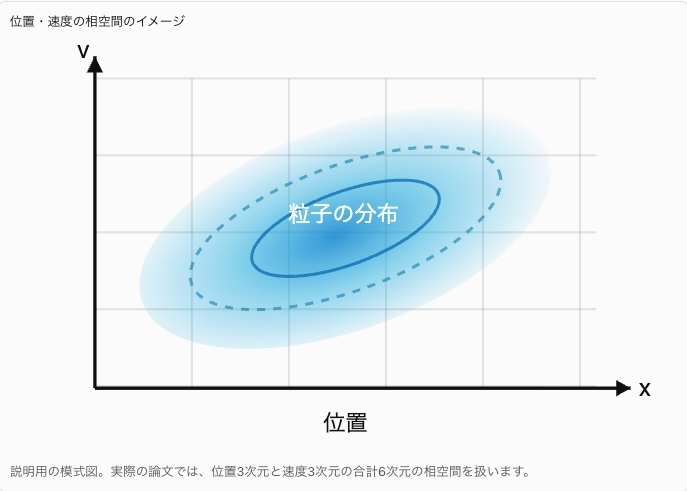
\includegraphics[width=.88\textwidth]{figures/phase_space.jpg}
\caption{位置・速度の相空間のイメージ。説明用の模式図であり、実際の論文では位置3次元と速度3次元の合計6次元の相空間を扱う。}
\label{fig:phase-space}
\end{figure}

分布関数を速度について積分すれば、密度や平均速度など、流体的な量を取り出せる。
1D1Vの場合、粒子密度 $n(x,t)$ と平均速度 $U(x,t)$ は
\[
n(x,t)=\int_{-\infty}^{\infty}f(x,v,t)\,\dd v,\qquad
U(x,t)=\frac{1}{n(x,t)}\int_{-\infty}^{\infty}v f(x,v,t)\,\dd v
\]
である（平均速度は $n>0$ の場所で定義する）。
3速度次元では積分を $\int_{\mathbb R^3}\dd^3v$ に置き換える。
Vlasov方程式を解くことで、密度だけでは区別できない速度分布の違いも追跡し、プラズマの波動、電場による加速、速度分布の変化などを調べられる。

\section{Maxwell分布と相対摂動 \texorpdfstring{$g$}{g}}
\subsection{平衡状態とは何か}
\textbf{平衡状態（equilibrium state）}とは、外部から新たな作用がなければ、時間が経過しても巨視的な状態が変化しない状態である。
本書で扱う論文では、特に空間的に一様で、平均流速がゼロのMaxwell速度分布を持つ状態を基準の平衡として採用する。

平衡状態でも、イオンは絶えずさまざまな方向へ運動し、その速度にはばらつきがある。
ある速度の粒子がある場所から出ていっても、周囲から同じ速度の粒子が入ってくれば、その場所の速度分布は変わらない。
個々の粒子は熱運動を続けていても、粒子全体の分布や密度・温度は時間的に変化しない。
したがって、平衡とは全ての粒子が静止することではない。

\subsection{平衡Maxwell分布とは何か}
Maxwell分布は、熱平衡にある粒子の速度分布を表す。
ここでは平均流速がゼロの平衡を考える。各速度成分はゼロを中心とするGaussian分布に従い、温度が高いほど分布の幅が広い。
これは速度ベクトルの分布であり、速さ $|\bm v|$ だけの分布とは区別する。
次元を持つ速度を $\bm V$ と書けば、イオンの平衡分布は
\[
f_0(\bm V)=n_0\left(\frac{m}{2\pi k_BT_i}\right)^{3/2}
\exp\left(-\frac{m|\bm V|^2}{2k_BT_i}\right)
\]
である。$n_0$ は平衡粒子密度、$m$ はイオン質量、$T_i$ はイオン温度、$k_B$ はBoltzmann定数で、$\int f_0\,\dd^3V=n_0$ を満たす。

熱速度 $v_{\mathrm{th}}=\sqrt{k_BT_i/m}$ を単位として $\bm v=\bm V/v_{\mathrm{th}}$ と置き、分布も $n_0/v_{\mathrm{th}}^3$ を単位として測る。
すると無次元の平衡Maxwell分布は
\begin{equation}
w(\bm v)=(2\pi)^{-3/2}\exp(-|\bm v|^2/2)
\label{eq:maxwell}
\end{equation}
となる。無次元とは、速度や分布を基準量との比で表すことで、物理単位を持たないという意味である。
この規約では $\int w\,\dd^3v=1$、各速度成分の分散は1であり、温度に由来する分布の幅は速度単位へ吸収されている。
温度の効果を取り除いたわけではなく、例えば後述する温度比 $\tau=T_i/T_e$ にも残る。

1速度次元への縮約では、対応する無次元平衡分布を
\[
\boxed{w_1(v)=\frac{1}{\sqrt{2\pi}}\ee^{-v^2/2}}
\]
と書く。図\ref{fig:maxwell-equilibrium}のように、速度0付近の粒子が多く、速度の絶対値が大きい粒子ほど少ない。
ただし、これは符号を持つ1成分の速度の分布であり、3次元の速さの分布を描いたものではない。
平衡状態ではこの分布の形が時間的に変化しない。

\begin{figure}[htbp]
\centering
% One-dimensional normalized Maxwell equilibrium (analytic curve).
\begin{tikzpicture}
\begin{axis}[
 width=.86\textwidth,height=5.8cm,
 xmin=-3,xmax=3,ymin=0,ymax=.45,
 xlabel={無次元速度 $v$},ylabel={平衡分布 $w_1(v)$},
 xtick={-3,-2,-1,0,1,2,3},ytick={0,.1,.2,.3,.4},
 grid=both,minor tick num=1,
 tick label style={font=\small},label style={font=\small}]
\addplot[blue!70!black,thick,domain=-3:3,samples=121]{exp(-x^2/2)/sqrt(2*pi)};
\end{axis}
\end{tikzpicture}

\caption{1速度次元の無次元Maxwell平衡分布。速度にはばらつきがあるが、平衡では曲線の形は時間に依存しない。表示範囲の外にも裾が続き、全速度での積分は1である。}
\label{fig:maxwell-equilibrium}
\end{figure}

\subsection{平衡からのずれを相対量で表す}
実際の分布を $f=f_0+\delta f$ と考え、平衡からの相対摂動を
\[
\boxed{g=\frac{f-f_0}{f_0}},\qquad \boxed{f=f_0(1+g)}
\]
と定義する。ここでは次元を持つ分布を使ったが、分子・分母を同じ単位で割れば比は変わらない。
以下では無次元化後の分布を改めて $f$ と書くので、同じ関係が $f=w(1+g)$ となる。

\begin{table}[htbp]
\centering
\caption{同じ位置・速度における $g$ の読み方。密度全体の増減率とは限らない。}
\begin{tabularx}{.92\textwidth}{lX}
\toprule $g$ の値 & 物理的な意味 \\\midrule
$0$ & 平衡分布と一致する。\\
$0.1$ & その位置・速度で平衡より10\%多い。\\
$-0.1$ & その位置・速度で平衡より10\%少ない。\\
$0.01$ & 平衡に対する1\%の小さな摂動である。\\
\bottomrule
\end{tabularx}
\end{table}

$g$ は無次元の相対的な分布の変化であり、密度そのものではない。
密度摂動は $g$ をMaxwell重み付きで速度積分した量である。
$g$ を用いると平衡は $g=0$ になり、平衡の周りの力学を一次項と二次項に整理し、Carleman線形化を適用しやすくなる。
ただし、点ごとの小さな $g$ と、後に用いるノルム条件 $R_P<1$ は同じ条件ではない。

\subsection{密度の揺らぎとKrook緩和}
1D1Vの場合は $f(x,v,t)=w_1(v)[1+g(x,v,t)]$ と書き、基準の平衡状態は
\[
\boxed{g(x,v,t)=0}
\]
である。一方、例えば周期領域で許される非ゼロ波数 $k$ に対して
\[
g(x,v,0)=0.1\cos(kx)
\]
とすると、$\int w_1\,\dd v=1$ より初期密度は
\[
n(x,0)=\int f(x,v,0)\,\dd v=1+0.1\cos(kx)
\]
となる。位置ごとに密度が平衡値より多かったり少なかったりするため、これは基準の一様平衡からずれた状態である。
この密度の揺らぎが電場を作り、その電場がさらに粒子の運動を変化させる。

後述するKrook緩和は、このような非平衡のずれを基準の平衡へ戻すモデルである。
輸送や電場など他の作用を無視すると、$\nuu>0$ の下で
\[
\partial_tg=-\nuu g,\qquad g(x,v,t)=g(x,v,0)\ee^{-\nuu t}
\]
なので、各位置・速度で
\[
\lim_{t\to\infty}g(x,v,t)=0,\qquad f(x,v,t)\longrightarrow w_1(v)
\]
となる。これは純粋な緩和だけを取り出した結論であり、一般の非線形発展には別途評価が必要である。

\subsection{平衡状態と定常状態の違い}
\textbf{定常状態（stationary state）}とは、時間が経過しても分布が変わらない状態である。
時間変化がないという性質だけでは、熱平衡にあるとは限らない。
例えば外部からエネルギーを供給し続けて一定の流れを維持する状態は、定常でも非平衡でありうる。

\begin{table}[htbp]
\centering\small
\caption{定常性、熱平衡、本書で採用する基準状態の区別。}
\begin{tabularx}{\textwidth}{lX}
\toprule 概念 & 意味 \\\midrule
定常状態 & 分布が時間に依存しない状態。外部駆動や流れがあっても定常になりうる。\\
熱平衡状態 & 熱力学的に平衡で、系と共に動く基準では持続的な熱流などがない状態。粒子の熱運動は続く。\\
本書の基準の平衡 & 平均流速ゼロの空間一様なMaxwell分布 $w(\bm v)$（1速度次元では $w_1(v)$）。\\
\bottomrule
\end{tabularx}
\end{table}

本書では、この特定の平衡を $g=0$ とすることがCarleman線形化への接続で重要になる。
平衡で時間微分がゼロになり、自己無撞着な電位もゼロになるため、Fourier--Hermite係数の方程式を
\[
\boxed{\dot\uu=F_1\uu+F_2(\uu\otimes\uu)}
\]
という定数項のない二次形式に整理できる。
Krook緩和によって平衡へ引き戻される効果と、非線形相互作用によって摂動が変わる効果を比較することで、後の章で収束の十分条件を導く。

\section{衝突付きVlasov方程式と自己無撞着な電位}
\sourcefile{HANDOVER.md} 第2節のモデルは、電子を断熱応答、イオンを運動論的に扱う、磁場なしの弱非線形プラズマである。
電子の密度応答は弱い電位について線形化し、イオン分布と電場の二次の相互作用を保持する。
空間は周期的で、衝突にはKrook型の緩和を用いる。
無次元方程式は
\begin{align}
\partial_t f&=-\bm v\cdot\nabla_x f
 +\nabla_x\phi\cdot\nabla_v f-\nuu(f-w),\label{eq:vlasov}\\
(\nabla_x^2-\tau)\phi&=-\int_{\mathbb R^3}g(\bm x,\bm v,t)w(\bm v)\,\dd^3v,
\qquad \tau=T_{\mathrm{ion}}/T_e>0.\label{eq:poisson}
\end{align}

式\eqref{eq:vlasov}は、分布 $f$ が空間輸送、電場加速、衝突緩和によってどう変わるかを表す。
符号を読みやすくするため、輸送と加速の項を左辺に移すと
\[
\partial_t f+\bm v\cdot\nabla_x f
+\bm a\cdot\nabla_v f=-\nuu(f-w),\qquad
\bm a=-\nabla_x\phi
\]
となる。衝突がなければ、粒子の軌道
\[
\frac{\dd\bm x}{\dd t}=\bm v,\qquad
\frac{\dd\bm v}{\dd t}=-\nabla_x\phi
\]
に沿って分布の値が運ばれる。
ここで $\phi$ は無次元静電ポテンシャルで、電場はこの規約で $\bm E=-\nabla_x\phi$ に対応する。
正のイオンに対する電荷・質量などの係数は無次元化に吸収されている。
右辺の $-\nuu(f-w)$ は、分布を基準のMaxwell分布へ戻す効果を表し、$\nuu>0$ は無次元緩和率である。

式\eqref{eq:poisson}は、分布から電位を決める遮蔽Poisson（Helmholtz）方程式である。
右辺の $\int gw\,\dd^3v$ は、平衡密度を1に規格化したときのイオン密度摂動である。
左辺の $-\tau\phi$ は電子の応答に由来する遮蔽を表す。
Fourier空間では、波数 $\bm k$ の密度摂動を $\rho_{\bm k}$ とすると
\[
\phi_{\bm k}=\frac{\rho_{\bm k}}{|\bm k|^2+\tau}
\]
となり、電位が密度摂動の線形汎関数であることがわかる。
分布から密度・電位を計算し、その電位を式\eqref{eq:vlasov}へ戻すため、この結合を\textbf{自己無撞着}と呼ぶ。
完全な平衡 $g=0$ なら、この周期系では $\phi=0$ である。
電位の符号や係数はこの無次元化に従い、別の規約を途中で混ぜると $F_1,F_2$ の符号も変わる。

\begin{notebox}
\textbf{「自己無撞着な電場」とは？}
粒子の分布が電場を決め、その電場が粒子の分布を変える関係を、矛盾なく同時に満たす電場のことである。
本モデルでは、各時刻の分布摂動 $g$ を速度について積分して密度摂動を求め、
式\eqref{eq:poisson}から電位 $\phi$、さらに電場 $\bm E=-\nabla_x\phi$ を計算する。
その電場による加速を式\eqref{eq:vlasov}へ入れて、分布を時間発展させる。
\[
\text{粒子分布}\ \longrightarrow\ \text{密度・電場}
\ \longrightarrow\ \text{粒子分布の変化}
\]
「自己」は粒子自身の分布が電場の源になること、
「無撞着」は分布から求めた電場と、分布の時間発展に使う電場が整合することを意味する。
ここでは電子の応答も遮蔽項を通じて含まれている。
このように、Vlasov方程式と遮蔽Poisson方程式を結合した問題として解く。
\end{notebox}

\subsection{相対摂動の方程式を導く}
式\eqref{eq:maxwell}より $\nabla_vw=-\bm v w$ なので、$f=w(1+g)$ の速度微分は
\[
\nabla_vf=(\nabla_vw)(1+g)+w\nabla_vg
=w\{-\bm v(1+g)+\nabla_vg\}
\]
である。$w$ は位置と時間に依存しないため、$\partial_tf=w\partial_tg$、$\nabla_xf=w\nabla_xg$ となる。
これらを式\eqref{eq:vlasov}へ代入し、$w$ で割ると
\begin{equation}
\boxed{\partial_tg=-\bm v\cdot\nabla_xg-\bm v\cdot\nabla_x\phi
 -(\bm v\cdot\nabla_x\phi)g+\nabla_x\phi\cdot\nabla_vg-\nuu g.}
\label{eq:g}
\end{equation}
五つの項は、空間輸送、平衡分布への電場作用、二つの非線形電場作用、衝突緩和に対応する。

\section{五つの項の物理的な意味}
\begin{table}[htbp]
\centering\small
\caption{式\eqref{eq:g}の各項。次数の分類は自己無撞着な電位 $\phi[g]$ を用いた場合である。}
\begin{tabularx}{\textwidth}{lXXc}
\toprule 項 & 名前 & 物理的な意味 & 次数 \\\midrule
$-\bm v\cdot\nabla_xg$ & 自由輸送 & 速度に従って粒子が移動する。 & 一次\\
$-\bm v\cdot\nabla_x\phi$ & 平衡分布への電場作用 & 電場が平衡速度分布を変形する。 & 一次\\
$-(\bm v\cdot\nabla_x\phi)g$ & 非線形電場作用① & 電場が既存の摂動分布にも作用する。 & 二次\\
$+\nabla_x\phi\cdot\nabla_vg$ & 非線形電場作用② & 加速が速度分布を移動・変形させる。 & 二次\\
$-\nuu g$ & 衝突緩和 & 摂動を平衡へ戻す。 & 一次\\
\bottomrule
\end{tabularx}
\end{table}

\subsection{第1項：自由輸送と位相混合}
電場と衝突がない1D1V系を考えると、
\[
\partial_tg=-v\partial_xg,\qquad
\partial_tg+v\partial_xg=0
\]
であり、解は
\[
\boxed{g(x,v,t)=g(x-vt,v,0)}
\]
である。速度 $v$ の分布は、その速度で空間を移動する。
例えば無次元速度 $v=2$ の成分は、無次元時間 $t=3$ で位置が6だけ進む（周期領域では位置を $L$ ごとに同一視する）。
異なる速度成分は異なる速さで進むため、相空間の分布はせん断され、位置を固定して見ると速度方向に細かな構造ができる。
これがphase mixing（位相混合）の基本である。
例えば初期状態が $g(x,v,0)=A\cos(kx)$ なら $g(x,v,t)=A\cos(kx-kvt)$ となり、速度に関する振動が時間とともに細かくなる。

\subsection{第2項：平衡分布への電場作用}
$-\bm v\cdot\nabla_x\phi$ は、電場が平衡Maxwell分布へ作用することから生じる。
実際、元の加速項の平衡部分は
\[
\frac{1}{w}\nabla_x\phi\cdot\nabla_vw=-\bm v\cdot\nabla_x\phi
\]
である。正のイオンが電場で加速されると、平衡速度分布からのずれが生まれる。
外から空間的に変化する電場を与える問題なら、初めに $g=0$ でもこの作用で摂動が生じる。
ただし本モデルの電位は外から任意に与えるものではなく、式\eqref{eq:poisson}で密度から決まる。
したがって全空間で $g=0$ の完全な平衡では $\phi=0$ となり、自発的に摂動が生まれるという意味ではない。
$\phi[g]$ が線形なので、この項も $g$ に関して一次である。

\subsection{第3項：電場と既存の摂動の相互作用}
$-(\bm v\cdot\nabla_x\phi)g$ は、第2項にさらに $g$ が掛かった項である。
$\nabla_v\{w(1+g)\}$ のうち $(\nabla_vw)g$ に由来し、電場が平衡から変形した分布へ作用する一部を表す。
電位は $g$ に対する線形な写像なので、電場と摂動の積は二次になる。
ここで「線形な写像」とは非局所的な速度積分・空間逆演算を含むことであり、各点で単純に $\phi=Cg$ とする意味ではない。

\subsection{第4項：加速による速度分布の移動・変形}
$+\nabla_x\phi\cdot\nabla_vg$ は、摂動自身の速度微分に由来する。
粒子の加速度 $\dd\bm v/\dd t=-\nabla_x\phi$ により、摂動は速度空間で運ばれる。
例えば局所的に一定の加速度 $a$ による速度輸送だけを取り出すと、$\partial_tg+a\partial_vg=0$ は速度を $at$ だけ移動させる。
本系では加速が位置と分布にも依存し、空間輸送と組み合わさって分布を変形させる。
この項も $\nabla_x\phi[g]$ と $\nabla_vg$ の積なので二次である。

第3項と第4項は、同じ加速作用をMaxwell分布基準で書き分けたものであり、両方が必要である。
第3項だけを残して第4項を落とすと元のVlasov方程式には対応しない。
次章では、この二つをまとめたときのHermite基底上の重要な相殺を示す。

\subsection{第5項：衝突緩和による指数減衰}
\textbf{Krook型の緩和（Krook relaxation）}とは、衝突などによって非平衡な速度分布が平衡Maxwell分布へ徐々に戻る効果を、単純な指数減衰で近似するモデルである。
衝突を詳細に計算する代わりに、平衡からのずれが単位時間当たり一定の割合で減少すると仮定する。
本書のモデルでは、その効果が式\eqref{eq:g}の $-\nuu g$ として現れる。

\section{Krook型緩和の仕組みと収束解析での役割}
\subsection{基本式：固定した平衡分布へ戻す}
式\eqref{eq:vlasov}の輸送・加速項を左辺へ移すと、
\[
\frac{\partial f}{\partial t}+\bm v\cdot\nabla_x f
-\nabla_x\phi\cdot\nabla_v f
=\boxed{C[f]=-\nuu(f-w)}
\]
となる。$f$ は現在の位置・速度の分布、$w$ は固定した平衡Maxwell分布、$\nuu>0$ は緩和率（無次元衝突周波数）である。
衝突項の作用だけを見ると、同じ位置・速度で $f>w$ なら分布を減らし、$f<w$ なら増やし、$f=w$ なら何も変えない。
これは速度空間の各点での平衡への復元であり、粒子数全体を自動的に保存するという意味ではない。

\subsection{指数減衰と緩和時間}
輸送と電場を無視し、時間に依存しない $w$ に対して $f=w(1+g)$ を代入すると
\[
w\frac{\dd g}{\dd t}=-\nuu w g,\qquad
\boxed{\frac{\dd g}{\dd t}=-\nuu g}
\]
を得る。したがって
\[
\boxed{g(t)=g(0)\ee^{-\nuu t}},\qquad
f(t)=w+\{f(0)-w\}\ee^{-\nuu t}.
\]
$g$ が正でも負でも、平衡からのずれの大きさが指数的に小さくなる。
緩和時間は
\[
\tau_{\mathrm{relax}}=\frac{1}{\nuu}
\]
であり、温度比 $\tau=T_i/T_e$ とは別の記号である。
$\nuu$ が無次元なので、この緩和時間も無次元の時間単位で表している。
今回のNumPy/SciPy実験では $\nuu=0.2$ なので $\tau_{\mathrm{relax}}=5$ となり、時間5で摂動は初期値の $\ee^{-1}\simeq0.368$、約36.8\%になる。

\begin{figure}[htbp]
\centering
% Analytic curve for pure Krook relaxation; not numerical experiment data.
\begin{tikzpicture}
\begin{axis}[
 width=.86\textwidth,height=6cm,
 xmin=0,xmax=5,ymin=0,ymax=1.05,
 xlabel={経過時間 $t/\tau_{\mathrm{relax}}=\nuu t$},
 ylabel={摂動の比 $g(t)/g(0)$},
 xtick={0,1,2,3,4,5},ytick={0,.2,.4,.6,.8,1},
 grid=both,minor tick num=1,
 tick label style={font=\small},label style={font=\small},
 legend style={font=\small,at={(.98,.98)},anchor=north east}]
\addplot[blue!70!black,thick,domain=0:5,samples=101]{exp(-x)};
\addlegendentry{$\exp(-t/\tau_{\mathrm{relax}})$}
\addplot[only marks,mark=*,red!70!black] coordinates {(1,0.3678794412)};
\draw[dashed,gray] (axis cs:1,0)--(axis cs:1,0.3678794412)--(axis cs:0,0.3678794412);
\node[anchor=south west,font=\small] at (axis cs:1.05,0.38) {$t=\tau_{\mathrm{relax}}$ で約36.8\%};
\end{axis}
\end{tikzpicture}

\caption{Krook緩和だけを取り出した場合の解析的な減衰曲線。横軸は緩和時間を単位とする経過時間、縦軸は非ゼロの初期摂動に対する比である。輸送・電場を含む数値実験の軌道ではない。}
\label{fig:krook-relaxation}
\end{figure}

\subsection{Carleman線形化の収束で重要な理由}
Fourier--Hermite展開後の二次ODEは
\[
\dot\uu=F_1\uu+F_2(\uu\otimes\uu)
\]
となり、Krook項は線形行列 $F_1$ に $-\nuu I$ として入る。
第3章で導くLyapunov変換後の行列は
\[
\widetilde F_1+\widetilde F_1^\dagger=-2\nuu I
\]
を満たす。線形系だけなら
\[
\frac{\dd}{\dd t}\normtwo{\tu}^2=-2\nuu\normtwo{\tu}^2
\]
となり、状態ノルムは減衰する。
一方、二次非線形作用はノルムの増幅に寄与する可能性がある。
そこで第4章では、非線形性と散逸性の比
\[
\boxed{R_P=\frac{\normtwo{\widetilde F_2}\normtwo{\tu_0}}{\nuu}}
\]
を用い、$R_P<1$ のとき非線形作用を散逸で抑えられるという十分条件を得る。
Krook緩和は、衝突の簡略化に加えて、この収束解析に使える明確な散逸を与える役割を持つ。
ただし、非線形系全体の解が常に純粋な $\ee^{-\nuu t}$ と同じ減衰等式を満たすという意味ではない。

\subsection{保存則と現実的な衝突演算子との違い}
Krookモデルは簡単に扱えるが、現実のクーロン衝突を完全に表現するものではない。
ここで用いるのは、緩和率が一定で、平衡分布 $w$ も固定されたモデルである。

\begin{table}[htbp]
\centering\small
\caption{本書の固定Maxwell分布型Krook緩和と、より詳細な衝突モデルの比較。計算負荷は離散化や実装にも依存する。}
\begin{tabularx}{\textwidth}{lXX}
\toprule 比較項目 & 本書のKrook型緩和 & より現実的な衝突演算子 \\\midrule
計算負荷 & 比較的小さい。 & 一般に大きくなる。\\
数学的構造 & 固定平衡への線形減衰。 & 速度微分・積分などを含む。\\
衝突の速度依存性 & 一定率モデルでは表さない。 & 考慮できる。\\
粒子数保存 & 一般には保存しない。 & 保存するよう構成できる。\\
運動量・エネルギー & 一般には保存しない。 & 適切な演算子では保存する。\\
Carleman収束解析 & 散逸を評価しやすい。 & 演算子に応じた追加の解析が必要。\\
\bottomrule
\end{tabularx}
\end{table}

例えば各位置で $n=\int f\,\dd^3v$、$\int w\,\dd^3v=1$ とすると、
\[
\int C[f]\,\dd^3v=-\nuu(n-1)
\]
であり、密度が平衡値と異なると衝突項だけでも変化する。
同様に、任意の速度モーメント $\psi(\bm v)$ について
\[
\int\psi(\bm v) C[f]\,\dd^3v
=-\nuu\left(\int\psi f\,\dd^3v-\int\psi w\,\dd^3v\right)
\]
となるため、一般に粒子数・運動量・エネルギーの保存則を満たさない。
ただし、周期境界で初期の総質量摂動がゼロなら、それをゼロに保つこととは矛盾しない。

分布自身の密度・流速・温度に合う局所Maxwell分布へ緩和させる保存型BGKモデルや、クーロン衝突に基づくLandau衝突演算子とは区別する必要がある。
これらへ置き換える場合には、保存則だけでなく、線形・非線形作用の構造や収束条件も改めて調べなければならない。

\subsection{無衝突系で収束を保証できるか}
本書の評価では $\widetilde F_2$ と $\tu_0$ を固定すると $R_P\propto1/\nuu$ なので、緩和率を小さくするほど十分条件は厳しくなる。
$\nuu=0$ ではこの指標は定義できず、Krook散逸に基づく保証をそのまま適用できない。

一方、無衝突Vlasov系にも位相混合があり、適切な条件ではLandau減衰が起こりうる。
これは分布が細かい速度構造を作ることで、電場や低次の観測量が減衰する現象であり、分布全体がKrook項によって一様に平衡へ戻ることとは異なる。
したがって、Landau減衰をそのまま $-\nuu I$ の代わりとして同じ証明に入れることはできない。

衝突による一様散逸だけに依存せず、観測量や適切なノルムを使ったLyapunov評価、Carlemanの収束条件を構成できるかは、次の研究課題である。
エネルギー保存系やHamilton系への適用を広げる方向にもつながるが、本プロジェクトでその保証を確立したわけではない。

\section{物理的な読み方と近似の階層}
自由輸送項は、速度によって異なる速さで空間構造が移動することを表す。
その結果、速度方向に細かい構造が生まれる位相混合を記述できる。
自己無撞着な電位は密度摂動から決まり、二次項がFourierモード間の相互作用を生む。
ただし、これらの現象を定量的に捉えるには十分な基底数が必要である。

本プロジェクトには三つの異なる近似がある。
第一に、物理モデル自体が磁場なし・弱電位・単純衝突を仮定する。
第二に、Fourier・Hermite基底を有限個に切り詰める。
第三に、有限ODEをCarleman階層の有限次数で近似する。
さらに時間積分の数値誤差が加わる。
Carleman解が基準ODE解に近づいても、元のPDEへのGalerkin収束や物理モデルの妥当性まで確認したことにはならない。

\begin{notebox}
実数の分布を扱っても、Fourier係数は複素数である。
内積には共役転置 $\dagger$ を用いる。$\uu^\dagger P\uu$ を $\uu^{\mathsf T}P\uu$ に置き換えてはいけない。
また、$f\geq0$ は $g\geq-1$ を意味するが、現行コードはこの非負性を検査していない。
\end{notebox}

\chapter{Fourier--Hermite展開から二次ODEを作る}
\begin{chaptergoal}
\cgitem 基底の正規化と添字の範囲を固定する。\\
\cgitem 非線形項のHermite相殺を計算する。\\
\cgitem 実装で使う $F_1,F_2$ の係数を得る。
\end{chaptergoal}

\section{1D1Vモデルの基底}
ここから第6章までは位置 $x\in[0,L)$、速度 $v\in\mathbb R$ の縮約系を扱う。
\textbf{Probabilists' Hermite多項式（確率論型Hermite多項式）}は、標準正規分布を重みとして直交する多項式の系列である。
Maxwell分布を基準とする速度方向の展開に適しており、速度による掛け算や微分を、係数間の簡単な行列演算へ置き換えられる。
以下では、Fourierの添字 $n$ と区別するため、Hermite次数には $a$ を使う。

\subsection{何を変換するのか：関数のPDEから係数のODEへ}
本論文で確率論型Hermite多項式を使う主な目的は、Maxwell分布を基準に速度依存性を展開し、Vlasov--Poisson偏微分方程式を有限次元の常微分方程式へ変換することである。
これは、Carleman線形化を適用するための前処理に当たる。
元の未知量 $g(x,v,t)$ は連続変数 $x,v,t$ に依存し、例えば自由輸送だけでも
\[
\partial_tg=-v\partial_xg
\]
というPDEを満たす。そこで位置と速度を基底展開し、時間依存性を係数に集める。

\begin{table}[htbp]
\centering\small
\caption{Fourier--Hermite展開で各変数をどう扱うか。}
\begin{tabularx}{\textwidth}{llX}
\toprule 変数 & 扱い & 目的 \\\midrule
位置 $x$ & Fourier展開 & 空間微分を波数との掛け算へ変換する。\\
速度 $v$ & Hermite展開 & 速度微分と速度による掛け算を係数間の行列演算へ変換する。\\
時間 $t$ & 連続変数として保持 & 係数のODEを解き、時間発展を求める。\\
\bottomrule
\end{tabularx}
\end{table}

速度方向だけなら、有限次数で
\[
g(v,t)\simeq\sum_{j=0}^{N_H}a_j(t)H_j(v)
\]
と近似する。最初の3項は
\[
g(v,t)\simeq a_0(t)+a_1(t)v+a_2(t)\frac{v^2-1}{\sqrt2}
\]
であり、時間依存する係数ベクトル $\bm a(t)=(a_0,a_1,a_2)^{\mathsf T}$ を未知量にできる。
無限個の基底を使う展開と異なり、有限個への切断は近似である。
次数を高くすると表現できる構造は増えるが、必要な次数は分布の滑らかさや位相混合の進み方に依存する。

\begin{figure}[htbp]
\centering
\begin{tikzpicture}[>=Stealth,
 stage/.style={draw,rounded corners,align=center,text width=10.8cm,minimum height=10mm},
 component/.style={draw,rounded corners,align=center,text width=2.7cm,minimum height=13mm},
 every node/.style={font=\small}]
\node[stage] (function) at (0,0) {速度の連続関数 $g(v,t)$};
\node[stage] (projection) at (0,-1.4) {Gaussian重み付き射影：$a_j(t)=\int_{\mathbb R}w_1(v)g(v,t)H_j(v)\,\dd v$};
\node[component] (density) at (-3.7,-3) {$a_0(t)$\\密度の摂動成分};
\node[component] (flow) at (0,-3) {$a_1(t)$\\運動量・流速に関係};
\node[component] (variance) at (3.7,-3) {$a_2(t)$\\速度分散に関係};
\node[stage] (vector) at (0,-4.6) {時間依存の係数ベクトル $\bm a(t)=(a_0,a_1,a_2)^{\mathsf T}$\\有限個の変数のODEを解く（$N_H=2$ の例）};
\draw[->] (function)--(projection);
\draw[->] (projection.south)--(density.north);
\draw[->] (projection.south)--(flow.north);
\draw[->] (projection.south)--(variance.north);
\draw[->] (density.south)--(vector.north);
\draw[->] (flow.south)--(vector.north);
\draw[->] (variance.south)--(vector.north);
\end{tikzpicture}

\caption{速度の連続関数から有限個の係数への変換。係数はGaussian重みの射影で得られる。密度・流速・速度分散との対応には、後述するモーメントの規格化が必要である。}
\label{fig:hermite-projection}
\end{figure}

\subsection{定義と最初の多項式}
確率論型Hermite多項式はRodriguesの公式
\[
\boxed{\mathrm{He}_a(v)=(-1)^a\ee^{v^2/2}
\frac{\dd^a}{\dd v^a}\ee^{-v^2/2}},\qquad a=0,1,2,\ldots
\]
で定義される。例えば $a=1$ では
\[
\mathrm{He}_1(v)=-\ee^{v^2/2}\frac{\dd}{\dd v}\ee^{-v^2/2}=v
\]
である。最初の6個を表\ref{tab:hermite-polynomials}に示す。

\begin{table}[htbp]
\centering
\caption{確率論型Hermite多項式。ここではまだ正規直交化していない。}
\label{tab:hermite-polynomials}
\begin{tabular}{cl}
\toprule 次数 $a$ & $\mathrm{He}_a(v)$ \\\midrule
0 & $1$\\
1 & $v$\\
2 & $v^2-1$\\
3 & $v^3-3v$\\
4 & $v^4-6v^2+3$\\
5 & $v^5-10v^3+15v$\\
\bottomrule
\end{tabular}
\end{table}

\subsection{確率論型と物理学型を区別する}
Hermite多項式には主に二つの規約がある。
表\ref{tab:hermite-conventions}のように、重みのGaussianの幅と多項式の係数が異なる。
\begin{table}[htbp]
\centering\small
\caption{確率論型と物理学型の比較。重みの規格化定数は省略した。}
\label{tab:hermite-conventions}
\begin{tabularx}{\textwidth}{lXX}
\toprule & 確率論型（Probabilists'） & 物理学型（Physicists'） \\\midrule
記号 & $\mathrm{He}_a(v)$ & $H_a^{\mathrm{phys}}(v)$\\
重み & $\ee^{-v^2/2}$ & $\ee^{-v^2}$\\
1次 & $v$ & $2v$\\
2次 & $v^2-1$ & $4v^2-2$\\
代表的な用途 & 確率統計、Gaussian重みの速度展開 & 量子調和振動子など\\
\bottomrule
\end{tabularx}
\end{table}
本書の1次元平衡Maxwell分布は標準正規分布
\[
w_1(v)=(2\pi)^{-1/2}\ee^{-v^2/2}
\]
であるため、確率論型が自然に対応する。
両者は $H_a^{\mathrm{phys}}(v)=2^{a/2}\mathrm{He}_a(\sqrt2v)$ で関係するが、規約を混ぜると後述する $\sqrt a$ などの結合係数が変わる。
本書の $H_a$ は物理学型の記号ではなく、次に定義する正規化済みの確率論型を意味する。

\subsection{Gaussian重みでの直交性と正規化}
最も重要な性質は、異なる次数がGaussian重みの内積で直交することである。
\[
\boxed{\int_{-\infty}^{\infty}w_1(v)\mathrm{He}_a(v)\mathrm{He}_b(v)\,\dd v
=a!\delta_{ab}},\qquad
\delta_{ab}=\begin{cases}1 & a=b,\\0 & a\ne b.\end{cases}
\]
例えば $\int w_1(v)\,v\,\dd v=0$ は左右対称な重みと奇関数の積の積分であり、
$\int w_1(v)v^2\,\dd v=1$ は標準正規分布の分散に対応する。
本書では
\[
\boxed{H_a(v)=\frac{\mathrm{He}_a(v)}{\sqrt{a!}}},\qquad
\boxed{\int_{\mathbb R}w_1(v)H_a(v)H_b(v)\,\dd v=\delta_{ab}}
\]
という正規直交化を使う。従って
\[
H_0=1,\quad H_1=v,\quad H_2=\frac{v^2-1}{\sqrt2},\quad
H_3=\frac{v^3-3v}{\sqrt6}
\]
となる。これらは多項式そのものであり、Gaussianを掛けたHermite関数とは区別する。

\begin{figure}[htbp]
\centering
% Orthonormal probabilists' Hermite polynomials; Gaussian weight is not plotted.
\begin{tikzpicture}
\begin{axis}[
 width=.86\textwidth,height=7cm,
 xmin=-2,xmax=2,ymin=-2.5,ymax=2.5,
 xlabel={無次元速度 $v$},ylabel={$H_a(v)$},
 xtick={-2,-1,0,1,2},ytick={-2,-1,0,1,2},
 grid=both,minor tick num=1,
 tick label style={font=\small},label style={font=\small},
 legend style={font=\small,at={(.5,-.23)},anchor=north,legend columns=2},
 domain=-2:2,samples=101]
\addplot[black,thick]{1};
\addlegendentry{$H_0=1$}
\addplot[blue!70!black,thick,dashed]{x};
\addlegendentry{$H_1=v$}
\addplot[red!70!black,thick,dashdotted]{(x^2-1)/sqrt(2)};
\addlegendentry{$H_2=(v^2-1)/\sqrt2$}
\addplot[green!50!black,thick,densely dotted]{(x^3-3*x)/sqrt(6)};
\addlegendentry{$H_3=(v^3-3v)/\sqrt6$}
\end{axis}
\end{tikzpicture}

\caption{正規化された確率論型Hermite多項式 $H_0$〜$H_3$。直交性は有限の表示範囲での通常の面積ではなく、全実数上でGaussian重みを掛けた内積について成り立つ。}
\label{fig:hermite-polynomials}
\end{figure}

\subsection{Fourier--Hermite係数への展開}
Fourier基底は $L^{-1/2}\ee^{\ii k_nx}$、$k_n=2\pi n/L$ とし、
\begin{equation}
g(x,v,t)\simeq\frac1{\sqrt L}\sum_{n=-N_F}^{N_F}\sum_{a=0}^{N_H}
u_{n,a}(t)\ee^{\ii k_nx}H_a(v),\qquad d=(2N_F+1)(N_H+1)
\label{eq:expansion}
\end{equation}
と展開する。式中の $u_{n,a}$ は全て同じベクトル $\uu$ の成分である。
実装では $n=-N_F,\ldots,N_F$ の順に、それぞれ $a=0,\ldots,N_H$ を並べる。
ゼロ始まりの添字は
\[
\operatorname{idx}(n,a)=(n+N_F)(N_H+1)+a
\]
となる。テンソル積の列添字は $i d+j$ であり、$u_i u_j$ に対応する。

実数条件とゼロ総質量摂動は
\begin{equation}
u_{-n,a}=u_{n,a}^*,\qquad u_{0,0}=0
\end{equation}
である。Krook緩和は一般に質量摂動を減衰させるが、初期にゼロならこのモードはゼロを保つ。
Hermite直交性から密度摂動には $a=0$ だけが寄与し、電位の係数は
\begin{equation}
\kappa_n=\tau+k_n^2,\qquad \phi_n=\frac{u_{n,0}}{\kappa_n}
\end{equation}
となる。$\tau>0$ なので $n=0$ にも逆演算の特異性はない。

\subsection{Hermite係数と速度モーメントの関係}
各位置での速度依存性を $g(x,v,t)=\sum_a c_a(x,t)H_a(v)$ と書けば、式\eqref{eq:expansion}の規約では
\[
c_a(x,t)=\frac1{\sqrt L}\sum_{n=-N_F}^{N_F}u_{n,a}(t)\ee^{\ii k_nx}
\]
である。直交性により $c_a=\int w_1gH_a\,\dd v$ として係数を取り出せる。
例えば速度だけを考え、最初の3項で近似すると
\[
g(v)=a_0H_0(v)+a_1H_1(v)+a_2H_2(v)
=a_0+a_1v+\frac{a_2}{\sqrt2}(v^2-1)
\]
となる。分布の速度依存性を基底と係数に分け、$(a_0,a_1,a_2,\ldots)$ を時間発展させればよい。

\begin{table}[htbp]
\centering\small
\caption{低次Hermite係数が記述する速度分布の特徴。係数と物理量の関係には密度による規格化などが入る。}
\begin{tabularx}{\textwidth}{lX}
\toprule 基底 & 関係する特徴 \\\midrule
$H_0=1$ & 粒子密度の変化。\\
$H_1=v$ & 平均流速・運動量の変化。\\
$H_2=(v^2-1)/\sqrt2$ & 温度・速度分散の変化。\\
$H_3=(v^3-3v)/\sqrt6$ & 熱流束に関係する高次モーメント。\\
$H_4$ 以降 & 高次モーメントや、より複雑な非Maxwell的構造。\\
\bottomrule
\end{tabularx}
\end{table}

各係数を平均流速・温度・熱流束そのものと同一視しないことが重要である。
実際、$f=w_1(1+g)$ に対して生の速度モーメント $M_j=\int v^j f\,\dd v$ は
\[
n=M_0=1+c_0,\qquad M_1=c_1,\qquad
M_2=n+\sqrt2c_2,\qquad M_3=3c_1+\sqrt6c_3
\]
となる（現れない高次係数は0とする）。
従って基底と係数の関係が一度わかれば、これらの物理モーメントを求めるたびに速度方向の数値積分を行う必要はない。
速度だけの展開 $g=\sum_j a_j(t)H_j$ なら、同じ式の $c_a$ を $a_a$ に置き換えればよい。
従って $n>0$ の場所の平均速度と速度分散は
\[
U=\frac{c_1}{n},\qquad
\sigma_v^2=\frac{M_2}{n}-U^2=1+\frac{\sqrt2c_2}{n}-U^2
\]
である。1次元の熱流束に関係する中心3次モーメントも
\[
\int(v-U)^3f\,\dd v=M_3-3UM_2+2nU^3
\]
なので、一般には $c_3$ だけでは決まらない。
基準平衡の周りの小さな摂動では、$c_1$ は流速、$\sqrt2c_2$ は速度分散の変化、$\sqrt6c_3$ は中心3次モーメントの主な一次寄与を表す。

\section{速度方向の相殺}
正規化したHermite多項式の微分は次数を一つ下げ、速度 $v$ による掛け算は隣接する二つの次数を結ぶ。
具体的には
\begin{align}
vH_a&=\sqrt{a+1}H_{a+1}+\sqrt a H_{a-1},\\
\partial_vH_a&=\sqrt a H_{a-1}
\end{align}
を満たす。これらは、多項式を微分・乗算した後に基底へ戻すための厳密な代数的恒等式である。
速度微分を速度格子の差分で近似する代わりに、係数間の疎な結合として表現できる。
ただし、有限の $N_H$ で外側の次数を捨てるGalerkin切断の誤差は残る。

\subsection{微分を行列に置き換える具体例}
$g=a_0H_0+a_1H_1+a_2H_2$ に対して、微分は
\[
\partial_vg=a_1H_0+\sqrt2a_2H_1
\]
である。基底 $(H_0,H_1,H_2)$ における微分後の係数は
\[
\partial_vg\quad\longleftrightarrow\quad
D\bm a,
\qquad D=\begin{pmatrix}0&1&0\\0&0&\sqrt2\\0&0&0\end{pmatrix},
\quad\bm a=\begin{pmatrix}a_0\\a_1\\a_2\end{pmatrix}
\]
となる。この場合の微分は次数を下げるので、3次元の基底内で厳密に閉じる。
一方、速度の掛け算は
\[
vg=a_1H_0+(a_0+\sqrt2a_2)H_1+\sqrt2a_1H_2+\sqrt3a_2H_3
\]
となり、上位の $H_3$ が生まれる。
$H_0,H_1,H_2$ の空間への射影を $\Pi_2$ と書くと
\[
\Pi_2(vg)\quad\longleftrightarrow\quad
V\bm a,\qquad
V=\begin{pmatrix}0&1&0\\1&0&\sqrt2\\0&\sqrt2&0\end{pmatrix}
\]
である。有限行列への置き換えで上位成分を捨てる箇所を明確にすると、代数的恒等式とGalerkin近似を区別できる。
空間方向も $\partial_x\ee^{\ii k_nx}=\ii k_n\ee^{\ii k_nx}$ なので、同じ基底内で空間微分を係数への掛け算にできる。

\subsection{二つの非線形電場作用をまとめる}
\begin{figure}[htbp]
\centering
\begin{tikzpicture}[>=Stealth,
 basis/.style={draw,rounded corners,minimum width=17mm,minimum height=9mm},
 every node/.style={font=\small}]
\node at (0,0) {$vH_a$:};
\node[basis] (mid) at (6.5,0) {$H_a$};
\node[basis] (lo) at (3,0) {$H_{a-1}$};
\node[basis] (hi) at (10,0) {$H_{a+1}$};
\draw[->,blue!70!black] (mid)--node[above] {$\sqrt a$}(lo);
\draw[->,blue!70!black] (mid)--node[above] {$\sqrt{a+1}$}(hi);
\node at (0,-1.4) {$\partial_vH_a$:};
\node[basis] (dm) at (6.5,-1.4) {$H_a$};
\node[basis] (dl) at (3,-1.4) {$H_{a-1}$};
\draw[->,blue!70!black] (dm)--node[above] {$\sqrt a$}(dl);
\node[align=center] at (0,-2.9) {$(-v+\partial_v)H_a$:};
\node[basis] (cm) at (6.5,-2.9) {$H_a$};
\node[basis] (ch) at (10,-2.9) {$H_{a+1}$};
\draw[->,red!70!black] (cm)--node[above] {$-\sqrt{a+1}$}(ch);
\node[align=center,text=gray] at (3,-2.9) {下向きは相殺};
\end{tikzpicture}

\caption{Hermite次数の結合。$a\geq1$ を描いた。$a=0$ では $\sqrt a=0$ となり下向きの結合はない。微分と速度乗算を組み合わせると、下向き結合が相殺される。}
\label{fig:hermite-coupling}
\end{figure}

二次項をまとめると
\[
-(v\partial_x\phi)g+(\partial_x\phi)\partial_vg
=(\partial_x\phi)(-v+\partial_v)g
\]
であり、
\begin{equation}
(-v+\partial_v)H_b=-\sqrt{b+1}H_{b+1}
\label{eq:hermitecancel}
\end{equation}
となる。下向きのHermite結合が相殺され、出力 $a$ には入力 $a-1$ が結合する。
この相殺済みの係数が \codeinline{build_plasma_1d()} に実装されている。
Hermite展開そのものが非線形性を消すわけではない。
Maxwell重みでの直交性と簡単な微分・乗算則により、非線形性を明示的な二次作用 $F_2$ に整理できることが、その後のCarleman線形化へつながる。

Fourier基底の積には
\[
(L^{-1/2}\ee^{\ii k_{n'}x})(L^{-1/2}\ee^{\ii k_{n''}x})
=L^{-1/2}(L^{-1/2}\ee^{\ii k_{n'+n''}x})
\]
という係数が生じる。これが非線形係数の $L^{-1/2}$ の由来である。
3空間次元の $L^{-3/2}$ をそのまま1次元へ持ち込まない。

\section{Galerkin方程式}
\subsection{Galerkin法の考え方：残差を基底に直交させる}
\textbf{Galerkin法（ガラーキン法）}は、未知関数を有限個の基底で近似し、元の方程式の残差が、その基底の張る空間に直交するように係数を決める方法である。
本書ではFourier--Hermite基底を使い、Carleman線形化へ渡す二次ODEを構成する。

まず単純なPDE $\partial_tg=\mathcal L[g]$ を考え、基底 $\psi_0,\ldots,\psi_N$ により
\[
g_N(x,t)=\sum_{j=0}^{N}a_j(t)\psi_j(x)
\]
と近似する。$g_N$ を元の方程式へ代入しても、有限個の基底では一般に全ての点で等式は成立しない。
そこで方程式の残差を
\[
R(x,t)=\partial_tg_N-\mathcal L[g_N]
\]
と定義し、
\[
\boxed{\langle\psi_m,R\rangle=0,\qquad m=0,\ldots,N}
\]
を課す。残差は $g_N-g$ という解の誤差そのものではなく、近似関数が元の方程式を満たさない度合いである。
Galerkin法は、この残差の基底空間への射影をゼロにする。
各格子点で残差をゼロにする選点法とは、条件の課し方が異なる。

\begin{figure}[htbp]
\centering
\begin{tikzpicture}[>=Stealth,every node/.style={font=\small}]
\draw[thick,gray] (-1,0)--(8,0) node[below left] {保持する基底空間};
\coordinate (origin) at (0,0);
\coordinate (action) at (5,2.8);
\coordinate (projected) at (5,0);
\draw[->,blue!70!black,very thick] (origin)--(action)
 node[midway,above left] {$\mathcal L[g_N]$};
\draw[->,green!40!black,very thick] (origin)--(projected)
 node[midway,below] {$\partial_tg_N=\Pi_N\mathcal L[g_N]$};
\draw[->,red!70!black,thick] (action)--(projected)
 node[midway,right] {$R$（基底空間に直交）};
\draw (4.7,0)--(4.7,.3)--(5,.3);
\fill (origin) circle (1.5pt);
\end{tikzpicture}

\caption{Galerkin条件の模式図。基底空間内にある $\partial_tg_N$ を、元の作用 $\mathcal L[g_N]$ の射影に一致させると、残差 $R=\partial_tg_N-\mathcal L[g_N]$ は基底空間に直交する。関数空間の関係を説明用の2次元図に置き換えている。}
\label{fig:galerkin-residual}
\end{figure}

時間に依存しない基底なら
\[
\sum_{j=0}^{N}\langle\psi_m,\psi_j\rangle\dot a_j
=\left\langle\psi_m,\mathcal L\left[\sum_{j=0}^{N}a_j\psi_j\right]\right\rangle.
\]
一般の基底では左辺に質量行列 $M_{mj}=\langle\psi_m,\psi_j\rangle$ が現れる。
正規直交基底なら $M=I$ なので
\[
\boxed{\dot a_m=
\left\langle\psi_m,\mathcal L\left[\sum_{j=0}^{N}a_j\psi_j\right]\right\rangle}
\]
となり、有限個の係数のODEが得られる。
同じ射影の考え方は非線形な作用にも適用できるが、得られるODEが線形になるとは限らない。

\subsection{Fourier--Hermite基底と重み付き内積}
1D1Vのプラズマ系では、位置の周期性に合わせて
\[
\psi_n(x)=\frac1{\sqrt L}\ee^{\ii k_nx},\qquad k_n=\frac{2\pi n}{L}
\]
を使い、速度にはMaxwell重みで正規直交する $H_a(v)$ を使う。
積基底を $\Psi_{n,a}(x,v)=\psi_n(x)H_a(v)$ と書き、内積を
\[
\boxed{\langle h,g\rangle=
\int_0^L\dd x\int_{\mathbb R}\dd v\,w_1(v)h(x,v)^*g(x,v)}
\]
と定義する。第1引数の複素共役を取る規約であり、$\langle\Psi_{n,a},\Psi_{m,b}\rangle=\delta_{nm}\delta_{ab}$ となる。
有限展開は
\[
g_N=\sum_{n=-N_F}^{N_F}\sum_{a=0}^{N_H}u_{n,a}(t)\Psi_{n,a}
\]
であり、その係数は $u_{n,a}=\langle\Psi_{n,a},g_N\rangle$ で得られる。
元の連続関数 $g$ から初期係数を作る場合も、同じ射影を使う。
ただし、時間発展後のGalerkin解が常に真のPDE解の射影と一致するとは限らない。

電位を式\eqref{eq:poisson}から消去して、摂動の右辺を $\mathcal G[g]$ とまとめれば、Galerkin条件は
\[
\boxed{\dot u_{n,a}=\langle\Psi_{n,a},\mathcal G[g_N]\rangle}
\]
である。$N_F=1,N_H=2$ なら保持する係数は $d=3\times3=9$ 個となる。
これは9個の複素係数の表現であり、実数の分布を表す共役対称性などを考えると、全てが独立な複素自由度ではない。
以下では式\eqref{eq:g}の五つの項を順に射影する。

\subsection{自由輸送の射影：同じ波数の隣接Hermite次数を結ぶ}
$\partial_x\psi_m=\ii k_m\psi_m$ を使うと
\[
-v\partial_xg_N=-\sum_{m,b}\ii k_m u_{m,b}\psi_m(vH_b)
\]
となる。Fourierの直交性は $m=n$ だけを残し、Hermiteの漸化式は
\[
\langle H_a,vH_b\rangle_{w_1}
=\sqrt{b+1}\delta_{a,b+1}+\sqrt b\delta_{a,b-1}
\]
を与える。出力側の次数 $a$ で整理すると
\[
\boxed{\left.\dot u_{n,a}\right|_{\mathrm{transport}}
=-\ii k_n\left(\sqrt{a+1}u_{n,a+1}+\sqrt a u_{n,a-1}\right)}.
\]
自由輸送はHermite次数を一つ上下に結合するが、Fourier波数 $n$ は変えない。
図\ref{fig:hermite-coupling}の速度乗算の結合が、ここでは $-\ii k_n$ を掛けた形で現れる。

\subsection{線形電場作用の射影：密度から一次モーメントへ}
直交性から $\int w_1H_a\,\dd v=\delta_{a0}$ なので、密度摂動は
\[
\rho(x,t)=\int w_1g_N\,\dd v=\sum_nu_{n,0}(t)\psi_n(x)
\]
となる。遮蔽Poisson方程式の各Fourier係数について
\[
(-k_n^2-\tau)\phi_n=-u_{n,0},\qquad
\phi_n=\frac{u_{n,0}}{\kappa_n},\quad\kappa_n=k_n^2+\tau
\]
を得る。$v=H_1(v)$ より
\[
-v\partial_x\phi=-\sum_n\ii k_n\frac{u_{n,0}}{\kappa_n}\psi_nH_1
\]
なので、
\[
\boxed{\left.\dot u_{n,a}\right|_{\mathrm{field}}
=-\ii\frac{k_n}{\kappa_n}u_{n,0}\delta_{a1}}.
\]
これは密度成分 $u_{n,0}$ が、電場を介して速度の一次モーメントに関係する成分 $u_{n,1}$ へ作用する結合である。
ここでもFourier波数は変わらない。

\subsection{二つの非線形項の射影：次数の相殺と波数の和}
二次項を $(\partial_x\phi)(-v+\partial_v)g_N$ とまとめ、式\eqref{eq:hermitecancel}を使うと
\begin{align*}
\partial_x\phi&=\sum_{n'}\ii k_{n'}\frac{u_{n',0}}{\kappa_{n'}}\psi_{n'},\\
(-v+\partial_v)g_N&=-\sum_{n'',b}\sqrt{b+1}\,u_{n'',b}\psi_{n''}H_{b+1}.
\end{align*}
速度方向の射影では $a=b+1$ だけが残り、下向きの結合は相殺される。
一方、空間方向の積は
\[
\boxed{\psi_{n'}\psi_{n''}=\frac1{\sqrt L}\psi_{n'+n''}}
\]
なので、射影後の波数は $n=n'+n''$ となる。
この二つを合わせると $a\geq1$ について
\[
\boxed{\left.\dot u_{n,a}\right|_{\mathrm{nonlinear}}
=-\frac{\ii\sqrt a}{\sqrt L}
\sum_{\substack{n'+n''=n\\|n'|,|n''|\leq N_F}}
\frac{k_{n'}}{\kappa_{n'}}u_{n',0}u_{n'',a-1}}
\]
を得る。$a=0$ では寄与はゼロとする。
係数同士の積 $u_{n',0}u_{n'',a-1}$ が、Galerkin系に残る二次非線形性である。
$n'=1,n''=1$ から $n=2$ が生じるように、新しいFourier波数を生成できる。
ただし、出力波数が保持範囲に入る場合だけ、その成分を有限ODEに残す。

\subsection{Krook緩和の射影と全体の方程式}
最後に緩和項は基底の直交性だけで
\[
\left.\dot u_{n,a}\right|_{\mathrm{collision}}
=\langle\Psi_{n,a},-\nuu g_N\rangle=-\nuu u_{n,a}
\]
となる。
式\eqref{eq:g}を基底に射影すると
\begin{align}
\dot u_{n,a}={}&-\ii k_n\bigl(\sqrt{a+1}u_{n,a+1}+\sqrt a u_{n,a-1}\bigr)
-\ii\frac{k_n}{\kappa_n}\delta_{a,1}u_{n,0}-\nuu u_{n,a}\notag\\
&-\frac{\ii\sqrt a}{\sqrt L}
\sum_{\substack{n'+n''=n\\|n'|,|n''|\leq N_F}}
\frac{k_{n'}}{\kappa_{n'}}u_{n',0}u_{n'',a-1}.
\label{eq:galerkin}
\end{align}
$a=0$ では最後の項をゼロとし、境界外の係数もゼロとする。
Fourier和が範囲外なら、その寄与を捨てる。端から反対側への折り返しは行わない。
この式には空間微分 $\partial_x$ も速度微分 $\partial_v$ も残っておらず、有限個の係数の積・和と時間微分だけがある。

これは閉じたGalerkin射影であり、添字を剰余で計算する離散畳み込みとは異なる。

係数をまとめれば
\begin{equation}
\boxed{\dot\uu=F_1\uu+F_2(\uu\otimes\uu)},\quad
F_1\in\mathbb C^{d\times d},\quad F_2\in\mathbb C^{d\times d^2}.
\label{eq:quadratic}
\end{equation}
例えば $N_H=2$ の各波数の線形ブロックは
\begin{equation}
F_{1,n}=-\nuu I-\ii k_n
\begin{pmatrix}
0&1&0\\
1+1/\kappa_n&0&\sqrt2\\
0&\sqrt2&0
\end{pmatrix}.
\label{eq:block}
\end{equation}
密度から $a=1$ への結合だけに電位の線形応答が加わるため、この行列は一般に対称ではない。
固定波数の状態を $\uu_n=(u_{n,0},u_{n,1},u_{n,2})^{\mathsf T}$ とすると、非線形項を省いた各行は
\begin{align*}
\dot u_{n,0}&=-\ii k_nu_{n,1}-\nuu u_{n,0},\\
\dot u_{n,1}&=-\ii k_n\left[\left(1+\frac1{\kappa_n}\right)u_{n,0}
+\sqrt2u_{n,2}\right]-\nuu u_{n,1},\\
\dot u_{n,2}&=-\ii k_n\sqrt2u_{n,1}-\nuu u_{n,2}
\end{align*}
である。密度、運動量、速度分散に関係する成分が互いに作用する構造を読み取れる。
この線形行列は波数ごとにブロック対角となり、異なるFourier波数の結合は二次作用に現れる。

二次行列の非ゼロ要素は、$n=n'+n''$、$a\geq1$ に対して
\begin{equation}
(F_2)_{\operatorname{idx}(n,a),\,\operatorname{idx}(n',0)d+\operatorname{idx}(n'',a-1)}
=-\frac{\ii\sqrt a\,k_{n'}}{\sqrt L\,\kappa_{n'}}.
\end{equation}
$F_2$ は二つの入力を区別する表現である。入力を交換した同じ係数を機械的に追加すると、二重計数になる。

\subsection{係数ベクトルからCarleman階層へ}
例えば $N_F=1,N_H=2$ では、係数を
\[
\uu(t)=\bigl(u_{-1,0},u_{-1,1},u_{-1,2},
u_{0,0},u_{0,1},u_{0,2},u_{1,0},u_{1,1},u_{1,2}\bigr)^{\mathsf T}
\]
という9成分のベクトルにまとめる。
式\eqref{eq:quadratic}の $F_1$ は自由輸送・線形電場作用・Krook緩和、$F_2$ は電場と分布摂動の二次相互作用を表す。
未知量が関数 $g$ から有限個の係数 $\uu$ になっても、二次非線形性は残っている。
さらにLyapunov変換と振幅規格化を施し、Carleman階層を有限次数で切断すると
\[
\boxed{\dot{\bm z}=A_C\bm z}
\]
という高次元の線形ODEを得る。
Fourier--Hermite展開がPDEから二次ODEへの変換、Carleman線形化が二次ODEから線形階層への変換を担い、これらが量子アルゴリズムへ接続する基盤となる。
有限のFourier・Hermite切断と有限のCarleman切断は、それぞれ異なる近似である。

\subsection{具体例：基本波から第2高調波が生じる}
初期状態 $g(x,v,0)=A\cos(k_1x)$ は速度に依存しない密度摂動であり、初期係数は
\[
u_{1,0}(0)=u_{-1,0}(0)=\frac{A\sqrt L}{2}
\]
だけが非ゼロである。
$N_F\geq2$、$N_H\geq1$ の場合、$n=2,a=1$ の非線形和には初期に $(n',n'')=(1,1)$ だけが寄与するので
\[
\boxed{\dot u_{2,1}(0)=-\frac{\ii k_1}{\sqrt L\kappa_1}
\left(\frac{A\sqrt L}{2}\right)^2
=-\frac{\ii k_1A^2\sqrt L}{4\kappa_1}}
\]
を得る。初期生成率は $A^2$ に比例し、$n=-2$ 側は複素共役となる。
最初に生成されるのはHermite次数1の成分であり、密度の第2高調波 $u_{2,0}$ の初期微分はゼロである。

\begin{figure}[htbp]
\centering
\begin{tikzpicture}[>=Stealth,every node/.style={font=\small},
 mode/.style={draw,rounded corners,align=center,text width=3.3cm,minimum height=14mm}]
\node[mode] (field) at (0,1) {密度 $u_{1,0}$\\電位 $\phi_1=u_{1,0}/\kappa_1$};
\node[mode] (perturbation) at (0,-1) {摂動 $u_{1,0}$\\Hermite次数0};
\node[draw,circle,minimum size=9mm] (product) at (3.5,0) {$\times$};
\node[mode] (output) at (7,0) {$\dot u_{2,1}(0)\ne0$\\波数 $1+1=2$\\Hermite次数 $0+1=1$};
\draw[->] (field.east)--(product.north west);
\draw[->] (perturbation.east)--(product.south west);
\draw[->] (product.east)--(output.west);
\end{tikzpicture}

\caption{二次の電場作用によるモード結合の例。電位を作る密度成分と摂動成分の積が、新しい波数と一つ上のHermite次数を生む。共役側では $(-1)+(-1)=-2$ となる。}
\label{fig:nonlinear-mode-coupling}
\end{figure}

線形系では各波数が閉じているため、初期にゼロの $n=\pm2$ は生成しない。
非線形系との差を確認するには少なくとも $N_F\geq2$ が必要であり、保存実験の $N_F=1$ ではこの生成先が射影で捨てられる。
第8章では、この解析式を使った高調波生成の検証を次の優先実験として挙げている。

\begin{exercise}[射影係数の確認]
初期密度摂動 $g(x,v,0)=A\cos(k_1x)$ のFourier係数と、$\dot u_{2,1}(0)$ を直接の射影計算で確かめよ。
自由輸送の射影で、入力次数 $b=a+1$ と $b=a-1$ がそれぞれ出力係数にどの係数で寄与するかを確認せよ。
また、非線形項の $L^{-1/2}$ がFourier基底の積から生じることを、空間内積を直接積分して確かめよ。
\end{exercise}

\subsection{有限射影で捨てるものと検証の順序}
元の分布は一般に無限個の基底係数を必要とするため、有限化によって表\ref{tab:galerkin-errors}の制約が生じる。
時間積分は射影そのものとは別の段階であり、その誤差も区別する。
\begin{table}[htbp]
\centering\small
\caption{有限Galerkin系と数値積分による主な制約。}
\label{tab:galerkin-errors}
\begin{tabularx}{\textwidth}{lX}
\toprule 原因 & 表現できない構造・生じる誤差 \\\midrule
Fourier打ち切り & 高波数の空間構造を保持できない。\\
Hermite打ち切り & 細かな速度分布や進行した位相混合を十分に表せない。\\
非線形項の射影 & 保持範囲外へ出るモード結合を捨てる。\\
時間積分 & 有限ODEを数値的に解く際に別の誤差が加わる。\\
\bottomrule
\end{tabularx}
\end{table}

Galerkin射影でまず確認すべきなのは、構成した $F_1,F_2$ が保持基底上で元の作用を正しく表すことである。
線形系で波数が混ざらないこと、二次項で解析式どおりに高調波が生成すること、実数分布の共役対称性が保たれることを調べる。
その上で $N_F,N_H$ を増やし、同じ物理的初期条件に対する観測量が収束するか確認する。
係数の式が正しいことと、有限解像度が対象現象に十分であることは別の検証である。

\begin{notebox}
Galerkin法は、PDEを保持基底上の有限ODEへ変えるが、二次非線形性は残す。
Lyapunov変換は、その有限ODEの座標を変え、散逸性と収束条件を評価しやすくする。
例えば本系では $P_{(n,a),(n,a)}=1+\delta_{a0}/\kappa_n$ により
$F_1^\dagger P+PF_1=-2\nuu P$ を得る。
Carleman線形化は、さらにテンソル階層へ埋め込むことで線形系を作り、有限次数で切断する。
この三つの操作の目的と近似誤差を分けて考える必要がある。
\end{notebox}

\section{速度方向にもFourier展開を使えるか}
速度方向をFourier基底で表現する方法もある。
Hermite基底を選ぶ理由は、本モデルの無限速度領域とGaussian平衡に適合し、低次モーメントや速度演算子を簡単に扱えるためである。
表\ref{tab:velocity-bases}では主に周期区間上のFourier級数と比較する。

\begin{table}[htbp]
\centering\small
\caption{速度方向のFourier表現とHermite表現。}
\label{tab:velocity-bases}
\begin{tabularx}{\textwidth}{lXX}
\toprule 比較項目 & 速度方向のFourier表現 & 本書のHermite展開 \\\midrule
適した領域 & 級数は周期的な速度区間。 & 無限速度領域とGaussian重み。\\
Maxwell分布 & 表現できるが、Maxwell重みで直交する基底ではない。 & 平衡のGaussian重みで直交する。\\
速度微分 & 速度波数との掛け算。 & 隣接する下位Hermite次数への結合。\\
速度 $v$ の掛け算 & 級数では一般にモード間結合。連続Fourier変換では波数微分に対応する。 & 隣接する上下Hermite次数への結合。\\
物理モーメント & 係数からの別途の計算が必要になりやすい。 & 低次係数から直接取り出せる。\\
\bottomrule
\end{tabularx}
\end{table}

連続Fourier変換は無限速度領域でも定義できるので、Fourier表現が無限領域を扱えないわけではない。
本書の選択はMaxwell重みと演算子構造への適合性によるもので、あらゆる問題でHermite基底が優れるという主張ではない。
位相混合により速度構造が細かくなると高次Hermite成分が必要になり、少数係数だけで常に高精度になるわけでもない。
Hermite展開は非線形性を消さず、明示的な二次作用 $F_2$ として整理してCarleman線形化へ渡す役割を持つ。

\section{NumPy/SciPyでHermite多項式を評価する}
SciPyの \codeinline{eval_hermitenorm} は、正規化前の確率論型Hermite多項式 $\mathrm{He}_a$ を計算する。
関数名の \codeinline{norm} は $\sqrt{a!}$ で規格化済みという意味ではないため、本書の $H_a$ を得るにはその係数で割る。
低次数の計算例は次のとおりである。
\begin{lstlisting}[language=Python]
import numpy as np
from scipy.special import eval_hermitenorm, factorial


def H(a, v):
    return eval_hermitenorm(a, v) / np.sqrt(factorial(a))


v = np.linspace(-3, 3, 100)
curves = [H(a, v) for a in range(4)]
for a in range(4):
    print(f"H_{a}(0.5) =", H(a, 0.5))
\end{lstlisting}
$v=0.5$ での値は順に約 $1$、$0.5$、$-0.530330$、$-0.561341$ である。
これは基底の描画や分布の再構成に使える例であり、現行のODE構築では多項式を速度点ごとに評価せず、上述の $\sqrt a$ などの結合係数を直接行列へ入れている。
高次数の評価では階乗の大きさや浮動小数点数の範囲にも注意が必要になる。

\chapter{自由エネルギーに合わせたLyapunov変換}
\begin{chaptergoal}
\cgitem 固有値と対数ノルムの違いを理解する。\\
\cgitem 密度モードを重くする $P$ が散逸性を示す理由を確認する。\\
\cgitem 線形系の減衰等式と非線形系の評価を分ける。
\end{chaptergoal}

\section{Carleman収束の保証に向けて安定性を見える形にする}
Galerkin法で得られた二次ODE
\[
\dot\uu=F_1\uu+F_2(\uu\otimes\uu)
\]
では、$F_1$ が自由輸送・線形電場作用・Krook緩和、$F_2$ が電場と分布摂動の非線形相互作用を表す。
Carleman線形化はこの系を高次テンソルの階層へ埋め込むが、有限次数で切断した近似が、次数を増やすだけで必ず元の解へ収束するとは限らない。
その保証には、線形部分の減衰と非線形作用による増幅の上界を比較する必要がある。

本論文でLyapunov変換を行う主な理由は、もともと線形作用に備わる安定性を、ノルムを使って明確に評価し、Carleman打ち切りの収束条件を構成することである。
変換が元の方程式へ新たな減衰や制御を加えるわけではない。
同じ物理的な時間発展を、安定性が見える座標・ノルムで測り直す操作である。
ただし、この変換だけで非線形近似の収束が保証されるわけではなく、初期振幅などの条件も必要になる。

\section{なぜ固有値だけでは足りないか}
非線形項を除いた線形系は
\[
\dot\uu=F_1\uu,\qquad \uu(t)=\ee^{tF_1}\uu(0)
\]
と解ける。有限次元では $F_1$ の全固有値の実部が負なら長時間で解はゼロへ近づく。
しかし、そのことからユークリッドノルムが全時刻で単調減少するとは限らない。
非正規行列では固有ベクトルが直交せず、一時的な増幅が起こりうる。
ノルムの瞬間的な増加率を支配するのは、Hermite部分の最大固有値
\begin{equation}
\mu_2(F_1)=\lambda_{\max}\left(\frac{F_1+F_1^\dagger}{2}\right)
\label{eq:lognorm}
\end{equation}
である。「対数ノルム」は $\log\normtwo{F_1}$ の意味ではない。
実際、
\[
\frac12\frac{\dd}{\dd t}\normtwo{\uu}^2
=\operatorname{Re}(\uu^\dagger F_1\uu)
\leq\mu_2(F_1)\normtwo{\uu}^2
\]
この関係は、積の微分を展開すると
\begin{align*}
\frac{\dd}{\dd t}\normtwo{\uu}^2
&=\dot\uu^\dagger\uu+\uu^\dagger\dot\uu\\
&=\uu^\dagger(F_1^\dagger+F_1)\uu
\leq2\mu_2(F_1)\normtwo{\uu}^2
\end{align*}
ということである。微分不等式を積分すれば
\[
\boxed{\normtwo{\uu(t)}\leq\ee^{\mu_2(F_1)t}\normtwo{\uu(0)}}
\]
を得る。スカラー系 $\dot x=-\gamma x$、$\gamma>0$ における
$|x(t)|=|x(0)|\ee^{-\gamma t}$ を、多変数の作用に対する上界へ拡張した形である。
\begin{table}[htbp]
\centering\small
\caption{線形系に対するユークリッド対数ノルムの読み方。}
\begin{tabularx}{\textwidth}{lX}
\toprule 対数ノルム & 保証・解釈 \\\midrule
$\mu_2(F_1)<0$ & 全ての初期方向で、ノルムの指数減衰を保証する。\\
$\mu_2(F_1)=0$ & ノルムが増えないことを保証するが、原点への収束までは示さない。\\
$\mu_2(F_1)>0$ & 一時的増幅がありうる。長時間で不安定とは限らない。\\
\bottomrule
\end{tabularx}
\end{table}
従って $\mu_2(F_1)<0$ ならユークリッドノルムでの一様な収縮を保証できる。
一方、$\mu_2(F_1)>0$ なら、Hermite部分の最大固有ベクトルの方向では初期のノルム増加率が正となる。
全ての初期状態が増幅するという意味ではなく、単調減衰を全方向に保証できないということである。

本プロジェクトの保存済み1D1V実験（$\nuu=0.2$）では、変換前の $\mu_2(F_1)=+0.05$ に対し、変換後は $\mu_2(\widetilde F_1)=-0.20$ である。
これは同じ線形系でも、元のユークリッドノルムでは見えなかった一様減衰が、変換後のユークリッドノルムで見えることを示す。
数値の詳細は第6章に示す。

\section{密度成分を重くする二次形式}
プラズマの自由エネルギーに対応する行列として
\begin{equation}
P_{(n,a),(n,a)}=1+\frac{\delta_{a,0}}{\kappa_n},\qquad
\mathcal F(\uu)=\frac12\uu^\dagger P\uu
\label{eq:pdef}
\end{equation}
を用いる。$\kappa_n>0$ なので $P$ は正定値である。
第1項は分布摂動の二乗ノルム、第2項は電位との結合に対応する密度成分の補正と読める。
ここでの $\mathcal F$ は二次自由エネルギーであり、後述する量子出力の運動エネルギーモーメントとは別の量である。

なぜ通常のノルムで構造が見えにくいのかを、$N_H=2$ の式\eqref{eq:block}で確認する。
$p_n=1+1/\kappa_n$ と置けば、共通の因子 $-\ii k_n$ を除いた結合は、$u_{n,0}$ から $u_{n,1}$ へは $p_n$、逆方向へは1である。
この非対称性に合わせ、密度成分 $a=0$ に重み $p_n$、$a\geq1$ の成分には重み1を与える。

\begin{figure}[htbp]
\centering
\begin{tikzpicture}[>=Stealth,every node/.style={font=\small},
 component/.style={draw,rounded corners,align=center,text width=2.5cm,minimum height=11mm}]
\node[anchor=east] at (-1.8,0) {元の座標};
\node[component] (density) at (0,0) {$u_{n,0}$\\密度成分};
\node[component] (velocity) at (6,0) {$u_{n,1}$\\一次速度成分};
\draw[->,blue!70!black] (density.north east) to[bend left=22]
 node[above] {$p_n=1+1/\kappa_n$} (velocity.north west);
\draw[->,blue!70!black] (velocity.south west) to[bend left=22]
 node[below] {$1$} (density.south east);
\node[anchor=east] at (-1.8,-2.5) {変換後};
\node[component] (td) at (0,-2.5) {$\tilde u_{n,0}=\sqrt{p_n}u_{n,0}$};
\node[component] (tv) at (6,-2.5) {$\tilde u_{n,1}=u_{n,1}$};
\draw[->,red!70!black] (td.north east) to[bend left=22]
 node[above] {$\sqrt{p_n}$} (tv.north west);
\draw[->,red!70!black] (tv.south west) to[bend left=22]
 node[below] {$\sqrt{p_n}$} (td.south east);
\end{tikzpicture}

\caption{密度成分と一次速度成分の結合。共通因子 $-\ii k_n$ を省いた係数を示す。密度成分を $\sqrt{p_n}$ 倍した座標では両方向の係数が一致する。}
\label{fig:lyapunov-coupling}
\end{figure}

式\eqref{eq:block}の移流・電場部分を $-\ii k_nB_n$ と書く。
密度成分の重み $p_n=1+1/\kappa_n$ に対し、$P_n=\operatorname{diag}(p_n,1,1)$ なら
\[
P_nB_n=
\begin{pmatrix}0&p_n&0\\p_n&0&\sqrt2\\0&\sqrt2&0\end{pmatrix}
=B_n^{\mathsf T}P_n.
\]
したがってこの部分は $P$ 内積では反Hermiteとなり、衝突項だけが二次形式を減らす。
一般の $N_H$ でも同じ隣接結合から
\begin{equation}
\boxed{F_1^\dagger P+PF_1=-2\nuu P}
\label{eq:lyapeq}
\end{equation}
を得る。これは数値的に未知の $P$ を探索した結果ではなく、モデルの構造に基づく具体的な $P$ の恒等式である。

\section{座標変換による散逸性の表示}
$S=P^{1/2}$ とおき、$\tu=S\uu$ とする。
すると
\begin{align}
\dot\tu&=\widetilde F_1\tu+\widetilde F_2(\tu\otimes\tu),\\
\widetilde F_1&=SF_1S^{-1},\qquad
\widetilde F_2=SF_2(S^{-1}\otimes S^{-1}).
\label{eq:transform}
\end{align}
$P$ は対角なので平方根は成分ごとに求められる。
式\eqref{eq:lyapeq}の左右に $S^{-1}$ を掛けると
\[
\widetilde F_1^\dagger+\widetilde F_1=-2\nuu I,
\qquad \boxed{\mu_2(\widetilde F_1)=-\nuu}.
\]
例えば式\eqref{eq:block}の変換後のブロックは
\[
\widetilde F_{1,n}=-\nuu I-\ii k_n
\begin{pmatrix}0&\sqrt{p_n}&0\\\sqrt{p_n}&0&\sqrt2\\0&\sqrt2&0\end{pmatrix}.
\]
線形部分は一様減衰とユニタリな回転の和になり、散逸の強さを直接読める。
固有値は相似変換で変わらないが、ノルムの測り方が変わる。

\subsection{一様散逸と反Hermite作用への分解}
$K=\widetilde F_1+\nuu I$ と置くと
\[
\boxed{\widetilde F_1=-\nuu I+K,\qquad K^\dagger=-K}
\]
となる。$K$ は反Hermite行列なので $\ee^{tK}$ はユニタリである。
\begin{table}[htbp]
\centering\small
\caption{変換後の線形作用の二つの成分。}
\begin{tabularx}{\textwidth}{llX}
\toprule 成分 & 性質 & ノルムへの作用 \\\midrule
$-\nuu I$ & 一様散逸 & 全ての方向を同じ割合で減衰させる。\\
$K$ & 反Hermite & 状態をユニタリに変化させ、ノルムを保つ。\\
\bottomrule
\end{tabularx}
\end{table}

$-\nuu I$ は $K$ と可換なので、線形系の解は
\[
\tu(t)=\ee^{-\nuu t}\ee^{tK}\tu(0)
\]
である。従って
\[
\frac{\dd}{\dd t}\normtwo{\tu}^2=-2\nuu\normtwo{\tu}^2,\qquad
\boxed{\normtwo{\tu(t)}=\ee^{-\nuu t}\normtwo{\tu(0)}}
\]
が厳密に成り立つ。
元の座標でも $\|\uu\|_P=(\uu^\dagger P\uu)^{1/2}$ と定義すれば、$\|\uu(t)\|_P$ が同じ割合で減衰する。
Lyapunov変換は、この $P$-ノルムによる記述を通常のユークリッドノルムへ移すものである。


\section{非線形項が残す三次の寄与}
線形系では式\eqref{eq:lyapeq}から厳密に
\begin{equation}
\frac{\dd\mathcal F}{\dd t}=-2\nuu\mathcal F,
\qquad \mathcal F(t)=\mathcal F(0)\ee^{-2\nuu t}
\end{equation}
が成り立つ。これは
\[
\frac{\dd\mathcal F}{\dd t}
=\frac12\uu^\dagger(F_1^\dagger P+PF_1)\uu
=-\nuu\uu^\dagger P\uu=-2\nuu\mathcal F
\]
と直接確認できる。
一方、二次非線形系では
\begin{equation}
\frac{\dd\mathcal F}{\dd t}
=-2\nuu\mathcal F+
\operatorname{Re}\{\tu^\dagger\widetilde F_2(\tu\otimes\tu)\}.
\label{eq:energycubic}
\end{equation}
第2項は状態について三次で、一般に符号一定ではない。
この項を上から評価して散逸に支配される範囲を求めるのが、次章の $R_P$ の役割である。
その見通しを先に示すと、$q(t)=\normtwo{\tu(t)}$ に対して $q>0$ のとき
\[
\dot q\leq\underbrace{-\nuu q}_{\text{線形散逸}}
+\underbrace{\normtwo{\widetilde F_2}q^2}_{\text{非線形作用の上界}}
\]
を得る。初期ノルムで両者を比較した量が
\[
R_P=\frac{\normtwo{\widetilde F_2}\normtwo{\tu_0}}{\nuu}
\]
であり、$R_P<1$ なら初期ノルム以下の領域が保たれ、
\[
q(t)\leq q(0)\ee^{-\nuu(1-R_P)t}
\]
と評価できる。次章では不変球と比較方程式によってこの評価を導く。
この減衰評価により、高次テンソルの大きさを制御する出発点が得られる。
Carleman全階層の打ち切り保証には、さらにbar座標での規格化や対応する定理の仮定が必要であり、線形部分の散逸性だけで十分とは言えない。

\section{変換なしでも計算できるか}
Galerkin ODEもCarleman行列も、元の座標のまま構成して数値計算できる。
可逆な座標変換は物理解を変更せず、線形行列の固有値も変えない。
同じCarleman次数を用いて初期状態と各ブロックを整合的に変換し、最後に元の座標へ戻せば、厳密演算では同じ近似を得る（第5章参照）。

\begin{table}[htbp]
\centering\small
\caption{座標変換で変わることと保たれること。散逸評価は本モデルの線形部分について記す。}
\begin{tabularx}{\textwidth}{lXX}
\toprule 比較項目 & 元の座標 & Lyapunov座標 \\\midrule
非線形ODEの物理解 & 変換して戻した解と同じ。 & 元の座標へ戻せば同じ。\\
線形行列の固有値 & 相似変換で不変。 & 元の行列と同じ。\\
ユークリッド対数ノルム & 正になる場合がある。 & $-\nuu$。\\
安定性の評価 & $P$-ノルムを用いて記述できる。 & ユークリッドノルムで直接記述できる。\\
収束条件 & rawのユークリッド評価だけでは不十分な場合がある。 & $R_P<1$ などの条件を評価しやすい。\\
同じ次数の物理座標の近似 & 整合的な変換の下で同等。 & 元の座標へ戻せば同等。\\
\bottomrule
\end{tabularx}
\end{table}

従って、変換が同じ次数の近似精度を必ず上げるわけではない。
主な価値は、物理的に適したノルムを同定し、そのノルムで散逸と非線形性を比較して収束条件を証明できることにある。
数値丸めや条件数の影響は、可逆変換による厳密な同等性とは別に検討する。

\section{拡張研究：正定値行列を選んで保証領域を広げられるか}
本論文では自由エネルギーに対応する具体的な $P$ を使う。
より一般には、Hermite正定値行列 $P$ と $\gamma>0$ に対して
\[
F_1^\dagger P+PF_1\preceq-2\gamma P
\]
を満たす組を探索することが考えられる。
$\preceq$ はHermite行列の半正定値順序を表す。
この不等式が成り立てば、変換後の対数ノルムは $\mu_2(P^{1/2}F_1P^{-1/2})\leq-\gamma$ となる。
固定した $P$ について利用できる最大の減衰率を
\[
\gamma(P)=-\lambda_{\max}\left(
\frac{P^{1/2}F_1P^{-1/2}+P^{-1/2}F_1^\dagger P^{1/2}}2\right)
\]
と定義し、$\gamma(P)>0$ の範囲を考える。
すると候補となる非線形性の指標は
\[
\boxed{R_P(P)=
\frac{\normtwo{P^{1/2}F_2(P^{-1/2}\otimes P^{-1/2})}
\normtwo{P^{1/2}\uu_0}}{\gamma(P)}}
\]
である。$\gamma(P)$ だけを大きくしても、同じ変換で非線形作用や初期ノルムが大きく評価されれば、この比が改善するとは限らない。
最適化する対象は、散逸率と変換後の非線形性を合わせた比になる。
また $P$ を正の定数倍しても、分子の二つの因子の倍率が相殺され、この指標は変わらない。

別の形の $P$ により同じ物理的初期状態に対する $R_P(P)$ を小さくできれば、十分条件が適用できる非線形領域を広げられる可能性がある。
これは本論文や現行NumPy/SciPy実装で実証した結果ではなく、そこから考えられる拡張研究である。
新しい $P$ の条件数、演算子構成の負荷、高次階層の規格化も含めて、実際に有用な保証になるかを検証する必要がある。


\begin{exercise}[変換の意味]
$S$ が可逆なとき、変換前後の非線形ODE解は $\tu(t)=S\uu(t)$ で対応することを確認せよ。
対数ノルムが改善したことを「同じ初期値問題の物理解が変わった」と解釈できない理由を述べよ。
\end{exercise}

\chapter{弱非線形条件と振幅規格化}
\begin{chaptergoal}
\cgitem $R_P$ をノルムの微分不等式から解釈する。\\
\cgitem $R_P<1$ が十分条件である意味を理解する。\\
\cgitem Lyapunov変換とbar座標への規格化を使い分ける。
\end{chaptergoal}

\section{解の安定性と近似の収束を分けて考える}
これから行う評価には二つの段階がある。
まず非線形ODE自身の解が、初期状態の周りの一定の球の外へ増大せず、時間とともに減衰することを示す。
次に、その性質と高次テンソルの規格化を用い、Carleman打ち切り次数を増やすと近似誤差が小さくなることを示す。
\[
\boxed{\text{非線形解の大きさを制御する}}
\quad\longrightarrow\quad
\boxed{\text{高次打ち切り誤差を制御する}}
\]
安定な非線形解が存在することと、ある打ち切り近似がその解へ収束することは同じ命題ではない。
本章は前者と規格化・有限階層の散逸性を、第5章は誤差伝播と後者の評価を扱う。
中心となる十分条件は $R_P<1$ だが、全階層の収束保証では、さらに規格化などの仮定を揃える必要がある。

\section{非線形性と散逸の比}
$q(t)=\normtwo{\tu(t)}$、$b=\normtwo{\widetilde F_2}$ とおく。
行列の $2$ ノルムは最大特異値であり、成分の二乗和の平方根（Frobeniusノルム）とは区別する。
式\eqref{eq:energycubic}のエネルギー微分を、ノルム $q$ で書き直すと
\begin{align*}
\frac12\frac{\dd}{\dd t}q^2
={}&\operatorname{Re}(\tu^\dagger\widetilde F_1\tu)\\
&+\operatorname{Re}\{\tu^\dagger\widetilde F_2(\tu\otimes\tu)\}.
\end{align*}
第1項は $-\nuu q^2$ に等しい。
第2項にはCauchy--Schwarz不等式と作用素ノルムの定義を使い、
\begin{align*}
\left|\tu^\dagger\widetilde F_2(\tu\otimes\tu)\right|
&\leq\normtwo{\tu}\,\normtwo{\widetilde F_2}\,
\normtwo{\tu\otimes\tu}\\
&=bq^3
\end{align*}
と評価する。ここでテンソル積の性質 $\normtwo{\tu\otimes\tu}=q^2$ を使った。
従って $\tfrac12\dd(q^2)/\dd t\leq-\nuu q^2+bq^3$ となり、$q>0$ なら $q$ で割って
\begin{equation}
\dot q\leq-\nuu q+bq^2.
\label{eq:riccatiineq}
\end{equation}
$q=0$ は平衡であり、右辺が多項式であるこのODEの解の一意性により、そのままゼロを保つ。
微分不等式の右辺は
\[
q(-\nuu+bq)
=\underbrace{-\nuu q}_{\text{線形散逸}}
+\underbrace{bq^2}_{\text{非線形作用の上界}}
\]
なので、$bq<\nuu$ の範囲では散逸が上界を上回る。
初期ノルムを $q_0=q(0)$ とおき、ここで
\begin{equation}
\boxed{R_P=\frac{bq(0)}{\nuu}}
\label{eq:rp}
\end{equation}
を導入する。$R_P<1$ なら、$q=q(0)$ の境界で右辺が負になるため、この球の内部が保たれる。
よって $q(t)\leq q(0)$ を再び代入すると
\begin{align}
q(t)&\leq q(0)\exp[-\nuu(1-R_P)t],\\
\frac{\mathcal F(t)}{\mathcal F(0)}&\leq\exp[-2\nuu(1-R_P)t].
\label{eq:energybound}
\end{align}
これが既存のエネルギー図に描かれている保守的な上界である。
$R_P$ が小さいほど強い減衰を保証し、1へ近づくほど保証される減衰率は小さくなる。
$bq^2$ は全入力方向を考えた上界であり、非線形項が実際に常に増幅に働くという意味ではない。

さらに比較方程式 $\dot y=-\nuu y+by^2$ を直接解くと
\begin{equation}
q(t)\leq\frac{q(0)\ee^{-\nuu t}}
{1-R_P(1-\ee^{-\nuu t})}\qquad (R_P<1)
\label{eq:sharperbound}
\end{equation}
も得られる。式\eqref{eq:energybound}は扱いやすさを優先した評価であり、実際の減衰が上界より速くても矛盾しない。

\section{十分条件の外側で何が言えるか}
$R_P\geq1$ では上の不変球による議論が使えない。
しかし $bq^2$ は全ての状態に対する最悪の上界であり、実際の軌道では非線形項の相殺や方向の効果がある。
したがって $R_P\geq1$ は、非線形解の発散、有限Carleman近似の失敗、あるいは物理的な強乱流の発生を意味しない。
逆に、一つの初期値が有限時間で減衰しても、全ての初期値に対する保証は得られない。

また $R_P$ は初期振幅だけでなく $N_F,N_H,L,\tau,\nuu$ に依存する。
実装の \codeinline{initial_state_for_r()} は固定テンプレート $\uu_{\mathrm{temp}}$ に対し
\[
\uu_0=\frac{R_{\mathrm{target}}\nuu}
{\normtwo{\widetilde F_2}\normtwo{S\uu_{\mathrm{temp}}}}\uu_{\mathrm{temp}}
\]
として目標値へ合わせる。物理パラメータを変えても $R_P$ を固定する掃引では、一般に物理的初期振幅も変わる。

\section{高次テンソルを制御するbar座標}
Lyapunov変換に続けて、非ゼロの初期値に対し
\begin{equation}
\bu=c\tu,\qquad c=\frac{1+R_{\mathrm{thr}}}{2\normtwo{\tu_0}},
\qquad 0<R_{\mathrm{thr}}<1
\label{eq:bar}
\end{equation}
と規格化する。このとき
\begin{equation}
\normtwo{\bu_0}=\frac{1+R_{\mathrm{thr}}}2<1,\quad
\overline F_1=\widetilde F_1,\quad
\overline F_2=\widetilde F_2/c.
\end{equation}
この規格化は $\normtwo{\bu^{\otimes j}}=\normtwo{\bu}^j$ を通じて高次成分の重みを制御する。
一方、
\[
\frac{\normtwo{\overline F_2}\normtwo{\bu_0}}{\nuu}
=\frac{\normtwo{\widetilde F_2}\normtwo{\tu_0}}{\nuu}=R_P
\]
なので、規格化そのものは非線形性と散逸の比を改善しない。
理論適用時に $R_P\leq R_{\mathrm{thr}}<1$ と選び、$r=(1+R_{\mathrm{thr}})/2$ とおけば、
$\normtwo{\bu(t)}\leq r<1$ なので
\[
\normtwo{\bu(t)^{\otimes j}}=\normtwo{\bu(t)}^j\leq r^j.
\]
高次成分自体は小さくなるが、これだけでは有限階層の誤差収束は証明できない。
階層間の結合が、打ち切りにより生じた誤差をどれだけ増幅するかも評価する必要がある。


提供資料の論文説明では、定理の適用時に $R_P\leq R_{\mathrm{thr}}<1$ を満たす閾値を選ぶ。
現行コードは $R_{\mathrm{thr}}=0.8$ を固定し、全ケースで $\normtwo{\bu_0}=0.9$ にする。
$R_P=1.2$ にも計算上の変換を施すが、この場合は上述の定理条件の外にある。
実装関数は $0<R_{\mathrm{thr}}<1$ のみを検査し、$R_P\leq R_{\mathrm{thr}}$ は検査しない。

\begin{warningbox}
$R_P$ は系と初期状態から計算する量、$R_{\mathrm{thr}}$ は規格化に用いる設定値である。
$R_{\mathrm{thr}}$ を下げると全階層誤差の数値が変わりうるが、それには測定座標の重みの変更も含まれる。
同じ物理状態に対する第1セクターの改善と、同じ意味で比較しない。
\end{warningbox}

\section{規格化された有限Carleman行列の散逸性}
第5章で構成する有限Carleman行列を $A_C$ と書く。
ここでは、その全ブロックをbar座標の $\overline F_1,\overline F_2$ で作ったものを考える。
$R_P\leq R_{\mathrm{thr}}<1$ の仮定の下で
\[
\bar b=\normtwo{\overline F_2}=\frac bc
=\frac{2\nuu R_P}{1+R_{\mathrm{thr}}}<\nuu
\]
となる。初期ノルムを小さくするだけでなく、階層の二次結合も散逸より弱くなる規格化である。

各次数 $j$ の対角ブロックは、線形作用のKronecker和なので
\[
\frac{A_{j,j}+A_{j,j}^\dagger}{2}=-j\nuu I,
\qquad \normtwo{A_{j,j+1}}\leq j\bar b
\]
を満たす。
有限階層の任意のベクトル $\bm v=(\bm v_1,\ldots,\bm v_N)$ に対し、$s_j=\normtwo{\bm v_j}$ と置くと
\begin{align*}
\operatorname{Re}(\bm v^\dagger A_C\bm v)
&\leq-\nuu\sum_{j=1}^{N}j s_j^2
+\bar b\sum_{j=1}^{N-1}j s_js_{j+1}\\
&\leq\sum_{j=1}^{N}\left[-j\nuu+\left(j-\frac12\right)\bar b\right]s_j^2\\
&\leq-\left(\nuu-\frac{\bar b}{2}\right)\sum_{j=1}^{N}s_j^2.
\end{align*}
2行目では $2s_js_{j+1}\leq s_j^2+s_{j+1}^2$ を使い、最上位の存在しない結合も上界として加えた。
$N=1$ でも同じ上界は成り立つ。
$\bar b<\nuu$ より、$\delta=\nuu-\bar b/2$ とすれば
\[
\boxed{\mu_2(A_C)\leq-\delta<-\frac{\nuu}{2}<0},
\qquad \normtwo{\ee^{tA_C}}\leq\ee^{-\delta t}
\]
を得る。これは全ての有限次数について成り立つ、保守的なブロックノルム評価である。
$R_P=1.2$ など定理の条件外で単にbar変換しただけの場合には、この議論をそのまま適用しない。
次章では、この指数作用の減衰を使って誤差の伝播を評価する。
\label{sec:finite-c-contractivity}

\section{数値実験で十分条件を判定する手順}
\begin{enumerate}
\item $N_F,N_H,\nuu,\tau,L$ と物理的な初期状態 $\uu_0$ を決め、$F_1,F_2$ を構成する。
\item 明示式で $P$ を作り、Lyapunov等式の残差を確認する。
\item $\widetilde F_1,\widetilde F_2$ を作り、$\gamma=-\mu_2(\widetilde F_1)>0$ を確認する。本モデルでは $\gamma=\nuu$ である。
\item $b=\normtwo{\widetilde F_2}$ を求める。小規模の密行列なら最大特異値をSVDで計算できる。
\item $q_0=\normtwo{P^{1/2}\uu_0}$ を計算し、$R_P=bq_0/\gamma$ を判定する。
\item $R_P<1$ なら、$R_P\leq R_{\mathrm{thr}}<1$ を満たす閾値を選び、bar座標で規格化する。
\item 第5章のような、対象とする誤差と全ての定数を含む上界から次数 $N_C$ を選ぶ。漸近式 $O(\log(1/\epsilon_C))$ だけでは具体的な整数次数は決まらない。
\end{enumerate}

保存実験の $\nuu=0.2$、$b\simeq0.3257350079$ を使えば
\[
\boxed{\normtwo{\tu_0}<\frac{0.2}{0.3257350079}\simeq0.6140}
\]
が十分条件となる。この数値は固定した基底数・物理パラメータに対するものである。
同じ $P,F_2,\uu_0$ を保って $\nuu$ を小さくすれば $R_P$ は大きくなり、この保証は厳しくなる。
目標 $R_P$ に合わせて初期振幅も変える既存の実験とは、比較条件を区別する。

\section{保証境界と実測収束、構造を使う改善の可能性}
$R_P=1$ は、この十分条件が使える範囲の境界であり、実際のCarleman収束の普遍的な境界ではない。
第6章の $R_P=1.2$ の保存結果では、$N_C=1$ から4へ増やすと第1セクター誤差は大幅に減少した。
これは特定の初期状態・有限時間・有限個の出力時刻での観測であり、全時刻の全階層収束を証明するものではない。

作用素ノルムによる評価は、$\widetilde F_2$ の入力として全ての $d^2$ 次元ベクトルを許した最悪ケースである。
実際の非線形入力は同じ状態の積 $\tu\otimes\tu$ であり、Fourier共役対称性、ゼロ総質量摂動などの制約もある。
例えば、それらが保たれる領域 $\mathcal D$ の全状態に対して
\[
\normtwo{\widetilde F_2(\bm v\otimes\bm v)}
\leq b_{\mathrm{eff}}\normtwo{\bm v}^2,
\qquad \bm v\in\mathcal D
\]
を正当化できれば、$R_{\mathrm{eff}}=b_{\mathrm{eff}}q_0/\gamma$ による、より鋭い安定性評価が考えられる。
ここでは $\bm v$ もLyapunov座標の状態であり、異なる座標のノルムを混ぜない。

ただし、観測した一本の軌道で小さい値を得ただけでは、領域全体に有効な定数にはならない。
さらに、元の状態の積に制限した上界を、そのままCarleman行列の任意の階層入力への作用素ノルムとして使うこともできない。
領域の不変性と、有限階層における誤差伝播を制御できることを別途示して初めて、打ち切りの収束保証を改善できる。
第3章の $P$ の選択の最適化と併せ、これらは今後の研究課題である。

\chapter{Carleman階層と打ち切り}
\begin{chaptergoal}
\cgitem 積の微分から線形の無限階層を導く。\\
\cgitem 有限次数で何を捨てるのかを具体化する。\\
\cgitem 対称テンソル圧縮と座標変換の意味を理解する。
\end{chaptergoal}

\section{基底の線形結合と方程式の線形化は別の操作}
\subsection{基底関数自身が一次関数である必要はない}
「関数を基底関数の線形結合で表すこと」と「非線形な時間発展方程式を線形方程式へ変換すること」は別の操作である。
例えば
\[
f(x)=x^2+3x+2
\]
は、$\varphi_0(x)=1$、$\varphi_1(x)=x$、$\varphi_2(x)=x^2$ と置けば
\[
f(x)=2\varphi_0(x)+3\varphi_1(x)+\varphi_2(x)
\]
と書ける。これは基底関数の線形結合だが、$\varphi_2$ 自身は $x$ の二次関数である。
一般に
\[
\boxed{f(x)=\sum_{j=0}^{N}a_j\varphi_j(x)}
\]
が線形結合というとき、係数 $a_j$ について足し算と定数倍で組み合わせることを意味し、$\varphi_j(x)$ が $x$ の一次関数であることは要求しない。
一次関数 $ax+b$ だけを何個線形結合しても、得られるのは高々一次の関数であり、一般の区間上の $x^2$ を正確には表せない。
数学的には $ax+b$ は一般にアフィン関数であり、厳密な線形写像は $b=0$ の場合を指すが、この区別も基底の線形結合とは別の話である。

\subsection{Fourier--Hermite展開後にも係数の積が残る}
本書の展開は式\eqref{eq:expansion}のとおり
\[
g_N(x,v,t)=\sum_{n=-N_F}^{N_F}\sum_{a=0}^{N_H}
u_{n,a}(t)\psi_n(x)H_a(v)
\]
である。右辺は $u_{n,a}$ を係数とする基底の線形結合であり、空間・速度について複雑な形の関数を表せる。
しかし、ここから得られる係数の時間発展は
\[
\boxed{\dot\uu=F_1\uu+F_2(\uu\otimes\uu)}
\]
という二次非線形ODEである。
元のVlasov方程式には電場と摂動の積があり、電位 $\phi[g]$ も摂動に線形に依存するため、射影後に $u_i u_j$ という係数の積が残る。
関数の変数 $x,v$ に対する形の複雑さと、時間発展の右辺が未知係数 $\uu$ に線形かどうかは、区別して考える必要がある。

\section{三つの操作の役割を整理する}
Fourier--Hermite展開とGalerkin射影は、連続関数を有限個の係数へ置き換える。
Lyapunov変換 $\tu=P^{1/2}\uu$ は、その係数の座標を変えて散逸性の評価をしやすくする。
変換後も
\[
\dot\tu=\widetilde F_1\tu+\widetilde F_2(\tu\otimes\tu)
\]
なので、二次非線形性は残る。
これに対しCarleman線形化は、高次の積そのものを新しい階層変数にして線形演算で表し直す。

\begin{table}[htbp]
\centering\small
\caption{関数表現、安定性評価、時間発展の線形化の違い。}
\begin{tabularx}{\textwidth}{lXX}
\toprule 手法 & 何を変換するか & 時間発展の非線形性 \\\midrule
Fourier--Hermite展開とGalerkin法 & 関数を有限個の係数へ置き換える。 & 二次の係数積が残る。\\
Lyapunov変換 & 安定性を評価しやすい座標へ移す。 & 二次非線形性が残る。\\
Carleman線形化 & 高次の積を階層の新変数として扱う。 & 無限階層として線形に表現し、有限打ち切りで近似する。\\
\bottomrule
\end{tabularx}
\end{table}

\begin{figure}[htbp]
\centering
\begin{tikzpicture}[>=Stealth,every node/.style={font=\small},
 stage/.style={draw,rounded corners,align=center,text width=11.3cm,minimum height=14mm}]
\node[stage] (pde) at (0,0) {非線形PDE：$\partial_tg=\mathcal L[g]+\mathcal Q[g,g]$\\位置・速度に依存する関数};
\node[stage] (ode) at (0,-2.2) {有限次元の非線形ODE：$\dot\uu=F_1\uu+F_2(\uu\otimes\uu)$\\係数の二次の積が残る};
\node[stage] (lyapunov) at (0,-4.4) {Lyapunov座標の非線形ODE：$\dot\tu=\widetilde F_1\tu+\widetilde F_2(\tu\otimes\tu)$\\散逸性の評価をしやすくする};
\node[stage] (carleman) at (0,-6.6) {高次元の線形ODE：$\dot{\bm z}=A_C\bm z$\\高次テンソルを階層変数にして有限次数で打ち切る};
\draw[->] (pde)--node[right] {Fourier--Hermite展開とGalerkin射影}(ode);
\draw[->] (ode)--node[right] {Lyapunov変換}(lyapunov);
\draw[->] (lyapunov)--node[right] {振幅規格化とCarleman線形化・打ち切り}(carleman);
\end{tikzpicture}

\caption{関数の基底展開と非線形方程式の線形化を順に使う流れ。Carlemanの有限系では、次元の増大と引き換えに線形の時間発展を得るが、打ち切り誤差も生じる。}
\label{fig:representation-vs-linearization}
\end{figure}

\section{テンソル積を新しい変数とする}
$\dot\bu=\overline F_1\bu+\overline F_2(\bu\otimes\bu)$ に対し、
$\bm w_j=\bu^{\otimes j}$ を新しい変数に取る。
例えば $j=2$ では積の微分により
\begin{align}
\dot{\bm w}_2={}&(\overline F_1\otimes I+I\otimes\overline F_1)\bm w_2\notag\\
&+(\overline F_2\otimes I+I\otimes\overline F_2)\bm w_3.
\end{align}
一般に
\begin{align}
\dot{\bm w}_j&=A_{j,j}\bm w_j+A_{j,j+1}\bm w_{j+1},\\
A_{j,j}&=\sum_{r=0}^{j-1}I^{\otimes r}\otimes\overline F_1\otimes I^{\otimes(j-1-r)},\\
A_{j,j+1}&=\sum_{r=0}^{j-1}I^{\otimes r}\otimes\overline F_2\otimes I^{\otimes(j-1-r)}.
\label{eq:carlemanblocks}
\end{align}
$A_{j,j}$ は $d^j\times d^j$、$A_{j,j+1}$ は $d^j\times d^{j+1}$ の行列である。
各式は階層変数について線形だが、上位の変数を必要とするため有限個では閉じない。
無限階層は元の解のテンソル積から厳密に得られる。ただし、任意の無限次元線形系としての解の存在・一意性には適切な関数空間の設定が必要である。

\section{有限階層を閉じる}
$N_C$ 次まで保持し、最上位の結合 $A_{N_C,N_C+1}$ を捨てる。
有限系の変数を $\bm z_j$ と書けば、一般に $t>0$ で $\bm z_j=\bu^{\otimes j}$ という厳密な積構造は保たれない。
例えば $N_C=3$ なら
\begin{equation}
\frac{\dd}{\dd t}
\begin{pmatrix}\bm z_1\\\bm z_2\\\bm z_3\end{pmatrix}
=\underbrace{\begin{pmatrix}
 A_{1,1}&A_{1,2}&0\\0&A_{2,2}&A_{2,3}\\0&0&A_{3,3}
\end{pmatrix}}_{A_C}
\begin{pmatrix}\bm z_1\\\bm z_2\\\bm z_3\end{pmatrix},\quad
\bm z_j(0)=\bu_0^{\otimes j}.
\end{equation}
解は $\bm z(t)=\ee^{tA_C}\bm z(0)$ であり、第1セクターを取り出して
\begin{equation}
\uu_C(t)=S^{-1}\bm z_1(t)/c
\label{eq:recover}
\end{equation}
とすれば物理係数の近似が得られる。
$N_C=1$ は二次項を捨てた線形系そのものである。
高次セクターの打ち切り誤差が下位へ伝わるので、第1セクターだけを見た誤差と全階層を見た誤差は異なる。

\section{安定性から全階層の打ち切り誤差へ}
\subsection{誤差は切り捨てた最上位結合から生まれる}
ここでは第4章の $R_P\leq R_{\mathrm{thr}}<1$ とbar規格化を仮定する。
厳密な非線形解のテンソル積を $N=N_C$ 次まで並べたベクトルを
\[
\bm w^{[N]}(t)=\begin{pmatrix}\bu(t)\\\bu(t)^{\otimes2}\\\vdots\\\bu(t)^{\otimes N}\end{pmatrix}
\]
とし、有限Carleman解を $\bm z^{[N]}$ と書く。
有限階層の $N=3$ の例では $\dot{\bm z}_3=A_{3,3}\bm z_3$ と閉じたが、厳密な $\bm w_3$ には $A_{3,4}\bm w_4$ の入力が残る。
一般に
\[
\dot{\bm w}^{[N]}=A_C\bm w^{[N]}+\bm f_N(t),\qquad
\bm f_N=\begin{pmatrix}0\\\vdots\\0\\A_{N,N+1}\bu^{\otimes(N+1)}\end{pmatrix}.
\]
この欠落した入力が打ち切り誤差の源であり、隣接ブロックの結合を通じて下位セクターにも影響する。
誤差 $\bm e_N=\bm z^{[N]}-\bm w^{[N]}$ に対しては
\[
\dot{\bm e}_N=A_C\bm e_N-\bm f_N(t),\qquad \bm e_N(0)=0
\]
となる。同じ初期テンソルを使うので、初期誤差はゼロである。
高次のテンソルが小さいだけでは十分ではなく、$A_C$ による誤差の伝播も制御する必要がある。

\subsection{本書で導ける保守的な全時間上界}
第4章で $r=(1+R_{\mathrm{thr}})/2<1$、$\bar b=\normtwo{\overline F_2}$、$\delta=\nuu-\bar b/2>\nuu/2$ と置いた。
非線形解の安定性と有限Carleman行列の散逸性から
\[
\normtwo{\bu(t)}\leq r,\qquad
\normtwo{\bm f_N(t)}\leq N\bar b\,r^{N+1},\qquad
\normtwo{\ee^{tA_C}}\leq\ee^{-\delta t}
\]
を得る。誤差方程式を定数変化法で積分すると
\[
\bm e_N(t)=-\int_0^t\ee^{(t-s)A_C}\bm f_N(s)\,\dd s
\]
なので、
\begin{align*}
\normtwo{\bm e_N(t)}
&\leq N\bar b\,r^{N+1}\int_0^t\ee^{-\delta(t-s)}\,\dd s\\
&=\frac{N\bar b}{\delta}r^{N+1}(1-\ee^{-\delta t}).
\end{align*}
従って
\begin{equation}
\boxed{\epsilon_C^{[N]}:=\sup_{t\geq0}\normtwo{\bm e_N(t)}
\leq\frac{N\bar b}{\delta}r^{N+1}}
\label{eq:full-convergence-bound}
\end{equation}
となる。これは本書のブロックノルム評価から導く保守的な補助上界であり、原論文の式そのものや、その定数を再掲したものではない。
$r<1$ などを固定すれば、$Nr^{N+1}$ は次数について指数的に小さくなり、目標精度に必要な次数は
\[
N_C=O\!\left(\log\frac1{\epsilon_C}\right)
\]
となる。例えば $r<\rho<1$ を固定すれば、$N(r/\rho)^N$ は有界なので $Nr^{N+1}$ を定数倍の $\rho^N$ で抑えられる。
ただし、$r\to1$ となるパラメータ変更まで同じ定数で保証するものではない。
原論文 Eqs.~(122)--(125) として提供資料で紹介される全階層の対数次数評価も、所定の収束・規格化条件の下での結果である。

\begin{notebox}
ここで全時間に対して評価したのは、bar座標の全階層誤差である。
第6章の数値指標は、有限時間の出力時刻で測った値であり、この上界や全時間の上限そのものではない。
また、一般の多変数系の誤差が $R_P^{N_C}$ になるとは述べていない。
次のスカラー例の幾何級数と、式\eqref{eq:full-convergence-bound}の $r^{N_C+1}$ は、意味と定数が異なる。
\end{notebox}

\section{スカラー系で確かめる}
理解のため $\dot x=-\gamma x+\beta x^2$、$x(0)=x_0$ を考える。
$\gamma>0$ を減衰率、$\beta$ を二次作用の係数とする。
新しい変数 $w_j=x^j$ を導入すると、積の微分から
\[
\dot w_j=jx^{j-1}\dot x=-j\gamma w_j+j\beta w_{j+1}
\]
を得る。最初の三つは
\begin{align*}
\dot w_1&=-\gamma w_1+\beta w_2,\\
\dot w_2&=-2\gamma w_2+2\beta w_3,\\
\dot w_3&=-3\gamma w_3+3\beta w_4.
\end{align*}
これを並べれば、無限次元だが
\[
\boxed{
\frac{\dd}{\dd t}\begin{pmatrix}w_1\\w_2\\w_3\\\vdots\end{pmatrix}
=\begin{pmatrix}
-\gamma&\beta&0&0&\cdots\\
0&-2\gamma&2\beta&0&\cdots\\
0&0&-3\gamma&3\beta&\cdots\\
\vdots&\vdots&\vdots&\vdots&\ddots
\end{pmatrix}
\begin{pmatrix}w_1\\w_2\\w_3\\\vdots\end{pmatrix}}
\]
という線形階層になる。
$w_j$ は元の $x$ から作った量なので、初期値には $w_j(0)=x_0^j$ という整合条件がある。
階層変数に関して右辺は線形でも、元の非線形系の全初期状態が任意の階層初期状態に対応するわけではない。
有限打ち切りでは $w_{N_C+1}$ への結合を落とすため、元の積構造とのずれが生じる。
元のスカラー方程式の厳密解は

\[
x(t)=\frac{x_0\ee^{-\gamma t}}
{1-(\beta x_0/\gamma)(1-\ee^{-\gamma t})}.
\]
$N_C=2$ の打ち切りなら
\[
z_2=x_0^2\ee^{-2\gamma t},\qquad
z_1=x_0\ee^{-\gamma t}
\left[1+\frac{\beta x_0}{\gamma}(1-\ee^{-\gamma t})\right].
\]
分母を幾何級数に展開した最初の二項が再現される。
一般に $N_C=N$ の第1成分は同じ級数の $m=0,\ldots,N-1$ の和となり、
$|\beta x_0|/\gamma<1$ なら全時刻で級数比を1未満に抑えられる。
\subsection{幾何級数の余りから次数を明示する}
ここからは $\beta>0,x_0>0$ に限定し、$R=\beta x_0/\gamma$、$0<R<1$ とする。
$N_C$ 次のCarleman系の第1成分を $x_{N_C}(t)$ と書けば
\[
\boxed{x_{N_C}(t)=x_0\ee^{-\gamma t}
\sum_{k=0}^{N_C-1}\left[R(1-\ee^{-\gamma t})\right]^k}
\]
である。厳密解との誤差は幾何級数の余りなので
\[
\boxed{|x(t)-x_{N_C}(t)|=
\frac{x_0\ee^{-\gamma t}\left[R(1-\ee^{-\gamma t})\right]^{N_C}}
{1-R(1-\ee^{-\gamma t})}}
\]
となる。$t\geq0$ では $0\leq1-\ee^{-\gamma t}<1$ なので
\[
\boxed{\sup_{t\geq0}|x(t)-x_{N_C}(t)|
\leq\frac{x_0}{1-R}R^{N_C}}
\]
を得る。従って絶対誤差を $\epsilon_C>0$ 以下にする十分な次数は
\[
\boxed{N_C\geq\max\left\{1,
\left\lceil\frac{\log\!\left(\dfrac{x_0}{(1-R)\epsilon_C}\right)}
{\log(1/R)}\right\rceil\right\}}
\]
である。$N_C\geq1$ の条件を付けることで、許容誤差が大きい場合も次数の定義と整合する。
$x_0$ と $0<R<1$ を固定した小さい目標誤差について、$N_C=O(\log(1/\epsilon_C))$ が具体的に確認できる。
これはスカラーの第1セクターに対する完全に計算できる例であり、多成分プラズマの全階層誤差の定理を、そのまま証明するものではない。

\section{次元増大と対称性}
無圧縮の状態次元は
\begin{equation}
D_{N_C}=\sum_{j=1}^{N_C}d^j
\end{equation}
である。疎行列化しても、状態ベクトル自体はこの長さを持つ。
一方、$\bu^{\otimes j}$ は添字の交換に対して対称であり、独立な次数 $j$ の単項式は $\binom{d+j-1}{j}$ 個である。
したがって対称基底なら
\begin{equation}
D_{N_C}^{\mathrm{sym}}=\sum_{j=1}^{N_C}\binom{d+j-1}{j}
\end{equation}
となる。$d=9,N_C=4$ では $7380$ 成分から $714$ 成分へ減らせる。
多重指数 $\bm m=(m_1,\ldots,m_d)$、$\sum_i m_i=j$ に対し
\[
\sqrt{\frac{j!}{m_1!\cdots m_d!}}\prod_i\bar u_i^{m_i}
\]
を対称成分とすれば、全テンソルのユークリッドノルムを保てる。
単に重複成分を一つだけ残す方法では全階層ノルムの重みが変わるので、圧縮前後の誤差比較には正規化が必要になる。
この圧縮は今後の課題であり、現行コードには実装されていない。

\section{可逆変換と打ち切りの整合性}
$T=cS$、$\mathcal T=\bigoplus_{j=1}^{N_C}T^{\otimes j}$ とすると、整合的に構成したraw座標とbar座標の有限Carleman行列は
\[
A_C^{\mathrm{bar}}=\mathcal T A_C^{\mathrm{raw}}\mathcal T^{-1}
\]
で対応する。階層ごとの変換なので最上位結合の切断とも整合する。
従って厳密演算では、同じ次数の近似を式\eqref{eq:recover}で戻した結果は一致する。
Lyapunov変換の利点は、物理解を変更することではなく、散逸性と収束を評価できるノルムを見つけることにある。
数値丸め・アルゴリズムの条件数により実際の計算では小さな差が生じうる。

\section{拡張の視点：どの基底で表現するか}
関数を表現する基底には、Fourier、Hermiteに加え、Chebyshev多項式、Legendre多項式、wavelet（ウェーブレット）、問題に合わせて学習した基底などの選択肢がある。
基底と切断の選び方により、同じ精度に必要な係数数、作用行列の疎性、モーメントや境界条件の扱いやすさが変わる。
少数の係数で対象の分布を十分に表せれば、Carleman階層の元の次元 $d$ も小さくできる可能性がある。

ただし、基底選択自体が時間発展の線形化やCarleman収束を保証するわけではない。
固定した線形な基底展開と射影では、もとの作用が二次なら係数についても二次の構造が保たれる。
この次数の保存はFourier--Hermite基底だけの性質ではないが、本系ではGaussian重みの直交性、微分・速度乗算の隣接結合、Fourier波数の和を使い、$F_1,F_2$ を具体的かつ構造的に書ける。
状態に応じて変わる基底や非線形な学習表現を使う場合は、追加の微分項や非多項式の依存性が生じうるため、係数方程式の構造を改めて確認する必要がある。

基底の変更による圧縮や疎化は、今後検討できる研究課題である。
その評価では、Galerkin誤差、初期状態の表現、Lyapunov評価、Carleman打ち切り誤差を分け、同じ物理的な問題と精度で比較することが必要になる。

\chapter{保存された数値実験を読む}
\begin{chaptergoal}
\cgitem 基準解、評価座標、正規化、評価時刻を確認する。\\
\cgitem 第1セクターと全階層の誤差を別々に読む。\\
\cgitem 小規模の成功例から結論できる範囲を定める。
\end{chaptergoal}

\section{実験条件と基準解}
保存データは $N_F=1$、$N_H=2$、$d=9$、$L=2\pi$、$\tau=1$、$\nuu=0.2$ に対応する。
時間は $[0,8]$ の等間隔101点、$R_P=0.2,0.7,1.2$、$N_C=1,2,3,4$ を比較している。
固定テンプレートには $n=\pm1$ の複数Hermite成分と $n=0$ の速度摂動が含まれ、各 $R_P$ に応じて全体振幅を変える。
純粋な密度余弦波のみの初期状態ではない。

基準解は同じ有限Galerkin ODEを \codeinline{solve_ivp(method="DOP853")} で積分したものとする。
許容誤差は \codeinline{rtol=1e-11, atol=1e-13}。
Carleman系にはCSR形式の疎行列と \codeinline{expm_multiply()} を使い、指数行列を密に生成せず、そのベクトルへの作用を計算する。
基準解は高精度の数値解であり、厳密解ではない。

\section{二種類の誤差と理論評価}
出力時刻集合を $\mathcal T=\{t_0,\ldots,t_{100}\}$ とする。
第1セクターの誤差は元の物理係数へ戻して
\begin{equation}
\widehat\epsilon_{\mathrm{first}}=
\max_{t_m\in\mathcal T}
\frac{\normtwo{\uu_C(t_m)-\uu_{\mathrm{ref}}(t_m)}}{\normtwo{\uu_0}}
\label{eq:firsterror}
\end{equation}
と定義する。分母は各時刻の解ノルムではなく、初期状態のノルムである。
減衰して小さくなった終状態に対する相対誤差とは意味が異なる。

全階層の誤差はbar座標の絶対誤差であり、
\begin{equation}
\widehat\epsilon_{\mathrm{full}}=
\max_{t_m\in\mathcal T}
\left(\sum_{j=1}^{N_C}
\normtwo{\bm z_j(t_m)-\bu_{\mathrm{ref}}(t_m)^{\otimes j}}^2\right)^{1/2}.
\label{eq:fullerror}
\end{equation}
初期状態で割る規格化はしていない。
$N_C$ が変わると比較する空間も増えるため、第1セクターと同じ速さで減る必要はない。
また、bar規格化を変更すれば各次数の重みが変わる。

提供資料が原論文 Eq.~(122) に対応づける量は、全階層に対する $\sup_{t\geq0}$ の誤差である。
式\eqref{eq:fullerror}は有限時間かつ有限個の時刻でしか評価していない。
時刻間で大きくなる誤差を捉えない可能性もあり、連続時間での最大値を保証する値ではない。
原論文の収束条件の下では、他の依存性を固定して $N_C=O(\log(1/\epsilon_C))$ という評価が紹介されているが、4点の次数比較だけからその漸近則を確認することはできない。

\section{線形構造と座標変換の照合}
\begin{table}[htbp]
\centering
\caption{\sourcefile{results/diagnostics.json} の保存値。}
\begin{tabularx}{\textwidth}{Xr}
\toprule 指標 & 保存値 \\\midrule
$\mu_2(F_1)$ & $+0.05$\\
$\mu_2(\widetilde F_1)$ & $-0.20$\\
Lyapunov等式の相対残差 & $0.0$\\
$\normtwo{\widetilde F_2}$ & $0.3257350079$\\
変換座標から戻した基準解との差（全ケースの最大） & $3.52\times10^{-12}$\\
\bottomrule
\end{tabularx}
\end{table}
対数ノルムの符号が変わることは、第3章で導いた構造と整合する。
残差の $0.0$ は保存された浮動小数点計算での値であり、一般のパラメータや別の演算順序で厳密にゼロになる保証ではない。
なお、\codeinline{lyapunov_residual()} のdocstringには無限大ノルムとあるが、実装は \codeinline{np.linalg.norm()} の既定値で行列のFrobeniusノルムを使う。
測っている値は
\[
\frac{\|F_1^\dagger P+PF_1+2\nuu P\|_{\mathrm F}}{\|2\nuu P\|_{\mathrm F}}
\]
である。これは関数の実際の計算に基づく定義である。

\section{第1セクターの収束}
\begin{table}[htbp]
\centering\small
\caption{式\eqref{eq:firsterror}の保存結果。CSVの値を有効数字6桁で丸めた。}
\begin{tabular}{rrrrr}
\toprule
$N_C$ & $D_{N_C}$ & $R_P=0.2$ & $R_P=0.7$ & $R_P=1.2$\\\midrule
1 & 9 & $8.09281\times10^{-3}$ & $2.83246\times10^{-2}$ & $4.85559\times10^{-2}$\\
2 & 90 & $1.29878\times10^{-6}$ & $1.59124\times10^{-5}$ & $4.67777\times10^{-5}$\\
3 & 819 & $1.15491\times10^{-8}$ & $4.95165\times10^{-7}$ & $2.49460\times10^{-6}$\\
4 & 7380 & $1.94297\times10^{-11}$ & $1.25894\times10^{-10}$ & $1.09067\times10^{-9}$\\
\bottomrule
\end{tabular}
\end{table}
第1セクターの誤差は急速に小さくなる。
ただし $10^{-11}$ 前後の値は、基準ODE解の誤差や指数作用計算の丸め誤差の影響も検討すべき領域である。
許容誤差を厳しくするなどの独立な検査なしに、表示された全桁をCarleman打ち切り誤差と断定しない。
$R_P=1.2$ でも誤差が減るのは、十分条件の外側にも良好な有限時間近似がありうることを示す一例である。

\begin{figure}[htbp]
\centering\includegraphics[width=.86\textwidth]{carleman_error.png}
\caption{保存済みの第1セクター誤差。物理座標へ戻し、初期状態ノルムで規格化している。}
\end{figure}

\section{全階層とエネルギーの挙動}
\begin{table}[htbp]
\centering\small
\caption{式\eqref{eq:fullerror}の保存結果。bar座標の絶対誤差。}
\begin{tabular}{rrrr}
\toprule $N_C$ & $R_P=0.2$ & $R_P=0.7$ & $R_P=1.2$\\\midrule
1 & $6.07643\times10^{-3}$ & $2.12674\times10^{-2}$ & $3.64579\times10^{-2}$\\
2 & $5.98574\times10^{-3}$ & $2.10082\times10^{-2}$ & $3.61213\times10^{-2}$\\
3 & $5.20589\times10^{-3}$ & $1.83218\times10^{-2}$ & $3.16037\times10^{-2}$\\
4 & $4.33786\times10^{-3}$ & $1.53036\times10^{-2}$ & $2.64714\times10^{-2}$\\
\bottomrule
\end{tabular}
\end{table}
全階層誤差は緩やかに減少する。初期barノルムが $0.9$ なので、高次のテンソル成分もまだ小さいとは言い切れない。
ただし、その事実だけで遅い減少の原因を完全に説明したことにはならない。
次数別の誤差寄与、異なる規格化、より高い $N_C$ を分けて測定する必要がある。

\begin{figure}[htbp]
\centering\includegraphics[width=.86\textwidth]{carleman_full_error.png}
\caption{保存済みの全階層誤差。第1セクターの図とは座標・正規化・対象が異なる。}
\end{figure}

保存された3ケースでは $\mathcal F$ は出力時刻上で単調減少し、$R_P<1$ の2ケースは式\eqref{eq:energybound}の上界と整合している。
$R_P=1.2$ では同じ保証は適用せず、実際の減衰を観測したと述べるにとどめる。
\begin{figure}[htbp]
\centering\includegraphics[width=.86\textwidth]{lyapunov_energy.png}
\caption{保存済みの二次自由エネルギーと保守的な上界。破線は $R_P<1$ のケースにのみ描く。}
\end{figure}

\section{今回のデータが検証していないこと}
$N_F=1$ では $n=\pm2$ の成分が表現できず、基本波から第2高調波への生成を観測できない。
既存の二次項は保持されたモード間で作用するが、物理的な非線形モード結合の十分な検証にはならない。
$N_H=2$ も小さく、長時間の位相混合やHermite切断境界からの影響を評価するには不足している。

基準ODEとCarleman解の一致は、共通の有限Galerkin方程式の比較である。
独立のPDE離散化、分布の非負性、Fourier・Hermite解像度の収束は別途調べる必要がある。
また古典的な小規模実験の速度や精度から、量子アルゴリズムの実行速度・実機資源・優位性を判断することはできない。

\chapter{量子アルゴリズムへの接続}
\begin{chaptergoal}
\cgitem 線形化の後にも残る演算子構成と読み出しの課題を知る。\\
\cgitem ブロックエンコーディングの規格化係数を理解する。\\
\cgitem 漸近的な高速化の主張を、その前提とともに読む。
\end{chaptergoal}

\section{巨大な線形系を量子状態へ}
Carleman系は線形だが、古典的に全成分を保存すれば $D_{N_C}$ の増大を避けられない。
量子計算では長いベクトルを振幅に符号化できるため、状態の添字自体には対数個の量子ビットを使える。
ただし入力準備、演算子の実装、時間発展、観測量の読み出しも効率的でなければ、状態表現の小ささは計算量の優位性につながらない。
本章は提供された論文解説に基づく理論の紹介であり、現行コードの機能ではない。

\section{ブロックエンコーディングの役割}
非ユニタリ行列 $M$ を直接量子ゲートとすることはできない。
補助量子ビットを加えたユニタリ $U_M$ の一部として
\begin{equation}
(\bra{0}^{\otimes a}\otimes I)U_M(\ket{0}^{\otimes a}\otimes I)
\simeq M/\alpha_M
\end{equation}
を実現する方法がブロックエンコーディングである。
$\alpha_M$ は少なくとも $\normtwo{M}$ 程度が必要で、アルゴリズムの反復回数などに影響する。
行列が大きいことだけでなく、どの構造を使って小さな規格化係数で構成できるかが重要になる。

遮蔽された電場の実空間相互作用は距離とともに減衰する。
階層的ブロックエンコーディングは、近距離を疎な相互作用として、遠距離を大きなブロックとして扱い、距離ごとの強度を構成へ反映する。
複数のユニタリの線形結合を実装するLCU法を使い、各階層を合成する。
提供資料では原論文 Eq.~(150) の結果として
\begin{equation}
\alpha_{\widetilde F_2}=O(\sqrt{N_FN_H}),\qquad
\alpha_{\widetilde F_1}=O(N_F\sqrt{N_H})
\end{equation}
が紹介される。固定した物理パラメータなどの依存性は省略されている。
単に現在の密な $F_2$ 配列を量子メモリへ格納すれば得られる評価ではない。

\section{履歴状態と観測量の推定}
量子ODEソルバは、時刻レジスタを含む履歴状態を準備する。
概念的には
\begin{equation}
\ket{\chi}\propto\sum_{s=0}^{M-1}
\normtwo{\bm z(s\Delta t)}\ket{\bm z(s\Delta t)}\ket{s},
\qquad \ket{\bm z(t)}=\frac{1}{\normtwo{\bm z(t)}}\sum_i z_i(t)\ket{i}
\end{equation}
と書ける。状態ベクトルの全成分を測定して復元すると、出力数に応じた大きな費用がかかる。
論文での目標は、時空間平均された非平衡運動エネルギーモーメントという指定された量の推定である。
高次積分近似と振幅推定を組み合わせ、時間平均と読み出しにかかる精度依存性も考慮する。

\begin{notebox}
現行コードが図示する $\mathcal F=\uu^\dagger P\uu/2$ は安定性評価に用いる二次形式である。
量子アルゴリズムの出力として紹介される運動エネルギーモーメントと、名称やグラフを取り違えない。
\end{notebox}

\section{計算量の比較を読む}
提供資料は、3D+3D系の代表的な比較として次の演算量を挙げている。
\begin{align}
\mathcal C_{\mathrm{op}}&=\widetilde O\left(
T N_F^4N_H^{7/2}\epsilon^{-1/p}\right),\\
\mathcal Q_{\mathrm{op}}&=\widetilde O\left(
N_FN_H^{1/2}\operatorname{polylog}(T/\epsilon)\epsilon^{-1}\right).
\end{align}
$\widetilde O$ は対数因子を省略し、$p$ は比較対象の古典的な陽的時間積分法の次数を表す。
古典メモリは $O(N_F^3N_H^3)$、量子ビット数は
\[
\widetilde O\left(\log(N_FN_H^{1/2}T)\log(1/\epsilon)\right)
\]
と紹介される。所定の弱非線形条件、初期状態準備、演算子アクセス、観測量の仮定に基づく漸近評価である。
1D1V実装の計算量を直接表す式ではない。

空間が高い正則性を持ち、速度方向のHermite正則性 $s_H=1$、$p=4$ の例では
\[
\mathcal Q_{\mathrm{op}}=\widetilde O(\epsilon^{-3/2}),\quad
\mathcal C_{\mathrm{op}}=\widetilde O(\epsilon^{-15/4}),\quad
\mathcal C_{\mathrm{op}}=\widetilde O(\mathcal Q_{\mathrm{op}}^{5/2})
\]
となる。これが「二次を超える高速化」という比較の意味である。
実際の定数、誤り訂正、入力データの準備費、比較する古典手法を含む実行時間の優位性は、この指数比較だけでは決まらない。

\section{保証される物理領域の狭さ}
提供資料には、原論文の代表条件 $\nuu=10^{-2}$ とDebyeスケールの分解能の下で、
無次元電位 $\varphi_{\max}$ の保証上限が単一Fourierモードで $7.12\times10^{-8}$、Gaussian密度摂動で $2.08\times10^{-5}$ と記載される。
同資料のトカマク炉心の典型値 $10^{-3}$〜$10^{-2}$ との隔たりは大きい。
これらは本プロジェクトの $\nuu=0.2$ の結果から得た閾値ではなく、一般の破綻点でもない。
また $\varphi$ と本書の $\phi$ の物理単位・温度基準を確認せずに直接比較してはいけない。
保証条件の保守性、磁場や現実的衝突演算子への拡張、より強い非線形現象への対応が研究課題として残る。

\chapter{再現手順と次の研究課題}
\begin{chaptergoal}
\cgitem 各関数と保存ファイルの役割を把握する。\\
\cgitem 既存結果を保持して数値実験を再現する。\\
\cgitem 非線形高調波を確認する実験を設計する。
\end{chaptergoal}

\section{コードと理論の対応}
\begin{table}[htbp]
\centering\small
\begin{tabularx}{\textwidth}{lX}
\toprule 実装の関数 & 役割 \\\midrule
\codeinline{build_plasma_1d} & 式\eqref{eq:galerkin}から $F_1,F_2,P$ を作る。\\
\codeinline{Plasma1D.transformed} & 式\eqref{eq:transform}の演算子を作る。\\
\codeinline{initial_state_for_r} & 初期テンプレートの振幅を目標 $R_P$ に合わせる。\\
\codeinline{r_number} & 式\eqref{eq:rp}の値を計算する。\\
\codeinline{logarithmic_norm} & Hermite部分の最大固有値を計算する。\\
\codeinline{lyapunov_residual} & Lyapunov等式の相対残差を計算する。\\
\codeinline{normalize_bar} & 式\eqref{eq:bar}の規格化を行う。\\
\codeinline{build_carleman_matrix} & 式\eqref{eq:carlemanblocks}の疎ブロックを組む。\\
\codeinline{solve_nonlinear} & 基準となる有限非線形ODEを積分する。\\
\codeinline{solve_carleman} & 指数作用で有限Carleman系を解く。\\
\codeinline{full_embedding_error} & 全階層の誤差を時刻上で集計する。\\
\bottomrule
\end{tabularx}
\end{table}
$F_1,F_2$ はNumPyの \codeinline{complex128} の密配列、$A_C$ はSciPyのCSR疎行列である。
$F_2$ のサイズは $d\times d^2$ なので、明示生成だけで $O(d^3)$ のメモリを要する。
行列の疎性や畳み込み構造を活用する最適化は、参照実装と照合しながら別途進める。

\section{実験の実行と保存物}
Python 3.11以上と \codeinline{uv} を用い、リポジトリルートで実行する。
以下は再現用のコマンドであり、本書で全スイープを再実行したことを意味しない。
\begin{lstlisting}[language=bash]
uv sync
uv run python -m unittest -v test_plasma_carleman
uv run python run_experiment.py \
  --nf 1 --nh 2 --nu 0.2 --tau 1.0 \
  --length 6.283185307179586 --tmax 8 --n-time 101 \
  --orders 1 2 3 4 --r-targets 0.2 0.7 1.2 \
  --outdir results/reproduction
\end{lstlisting}
出力先を別ディレクトリにすれば、本書が参照する既存結果を保持したまま比較できる。
\sourcefile{HANDOVER.md} によると2026年10月18日に7件の既存テストが成功しているが、その記録と保存された全実験の生成時点は区別する。

\sourcefile{error_by_order.csv} は次数、次元、第1セクター誤差、全階層誤差を持つ。
\sourcefile{diagnostics.json} はモデル設定、Lyapunov残差、対数ノルム、変換解の一致、エネルギー検査を持つ。
\sourcefile{energy_timeseries.npz} は時刻と規格化済みエネルギーなどを保存する。
3枚のPNGはCSVや時系列の可視化である。
現行の記録だけではライブラリ版、Gitコミット、全ての設定を完全に特定できないため、今後はそれらも同時に保存することが望ましい。

\begin{warningbox}
現行 \codeinline{solve_carleman()} は入力 \codeinline{times} の先頭・末尾・点数から等間隔の出力時刻を作る。
非等間隔の内部点は反映されない。
また指数作用は $\ee^{tA_C}\bm z_0$ の時刻 $t$ を使うため、基準ODEとの比較は本書のように開始時刻を0にする。
非ゼロ時刻で与えた初期値を扱うには、時間原点の整合性も修正する必要がある。
\end{warningbox}

\section{P0：第2高調波を確認する}
最優先の次期課題は、$N_F\geq2,N_H\geq2$ として非線形ODEのみを使い、$g(x,v,0)=A\cos(k_1x)$ からの高調波生成を調べることである。
この段階では巨大なCarleman行列を作る必要はない。
初期係数は $u_{\pm1,0}=A\sqrt L/2$、それ以外はゼロにする。
式\eqref{eq:galerkin}より、
\begin{equation}
\boxed{\dot u_{2,1}(0)=-\frac{\ii k_1}{\sqrt L\kappa_1}
\left(\frac{A\sqrt L}{2}\right)^2
=-\frac{\ii k_1A^2\sqrt L}{4\kappa_1}.}
\label{eq:harmonic}
\end{equation}
$n=-2$ の微分はその複素共役となる。
線形系はFourier波数ごとに閉じるので、$F_2=0$ にした対照系では初期にゼロの $n=\pm2$ は生成しない。

観測量として
\[
M_n(t)=\left(\sum_{a=0}^{N_H}|u_{n,a}(t)|^2\right)^{1/2}
\]
を記録する。小さい時間では $M_2(t)=|\dot u_{2,1}(0)|t+O(t^2)$ となり、初期生成率が $A^2$ に比例する。
密度の第2高調波 $u_{2,0}$ は初期微分がゼロなので、$a=1$ の生成より遅れて現れる点にも注意する。
複数振幅で解析式と比較し、共役対称性、ゼロ総質量、時間積分の収束性を検査する。
これらは今後実装する受け入れ基準であり、既存の成果ではない。

\section{P1：保証と実測収束の差を測る}
$\nuu,\tau,N_F,N_H$、初期形状と振幅を掃引し、$R_P$ と誤差・エネルギー・計算時間・メモリを記録する。
実験は二系統に分ける。
一つは同一 $R_P$ に振幅を合わせ、定理の指標に沿って比較するもの。
もう一つは物理的な初期振幅を固定し、条件変更による $R_P$ の変化も含めて測るものである。
$\max|\phi|$ など物理振幅も併記すると、単一のノルム指標だけに依存しない解釈ができる。

誤差を小さくする際は基準ODEの許容誤差も変え、参照解の精度が十分か確認する。
raw・tilde・bar座標を同じ次数で構成して物理座標へ戻す比較も行えば、実装の相似変換整合性を検証できる。

\section{P2・P3：高次化と物理的検証}
P2では第5章の正規化済み対称基底を実装し、小規模問題で無圧縮系と解・全階層ノルムを照合する。
引継書の目標は従来解との相対誤差 $10^{-9}$ 以下と、実測メモリ・時間の比較である。
行列フリー作用も候補だが、指数作用計算が必要とする随伴作用やtraceの扱いを含めて設計する必要がある。

P3では独立な $x$--$v$ 格子法との比較、$N_F,N_H$ の解像度収束、分布の非負性を確認し、その後に1D2Vや2D2Vなどへの拡張を検討する。
例えば $N_F=2,N_H=2$ では $d=15$、$N_C=4$ の無圧縮状態は54240成分になる。
条件を一度に大きくせず、解析可能な生成率や構造保存を基準に拡張することが、次の理論・量子実装を支える。

\appendix
\chapter{記号・検証・演習の補足}
\section{記号表}
\par\noindent
\begin{tabularx}{\textwidth}{lX}
\toprule 記号 & 意味 \\\midrule
$f,w,g$ & 分布関数、平衡Maxwell分布、相対摂動 $f=w(1+g)$。\\
$\phi,\tau,\nuu$ & 無次元電位、イオン・電子温度比、Krook緩和率。\\
$N_F,N_H,N_C$ & Fourier、Hermite、Carlemanの打ち切り次数。\\
$k_n,\kappa_n$ & 波数 $2\pi n/L$、遮蔽係数 $\tau+k_n^2$。\\
$\uu,F_1,F_2$ & 有限Galerkin係数、一次作用、二次作用。\\
$P,S$ & 自由エネルギーの正定値行列、平方根 $S=P^{1/2}$。\\
$\tu,\bu$ & Lyapunov座標 $S\uu$、振幅規格化座標 $cS\uu$。\\
$R_P,R_{\mathrm{thr}}$ & 非線形性と散逸の比、bar規格化用の閾値。\\
$\bm w_j,\bm z_j$ & 厳密解の $j$ 次テンソル、有限Carleman系の第 $j$ セクター。\\
$\mu_2,\normtwo{\cdot}$ & ユークリッド対数ノルム、ベクトル2ノルム／行列最大特異値。\\
$D_{N_C}$ & 無圧縮Carleman状態次元 $\sum_{j=1}^{N_C}d^j$。\\
\bottomrule
\end{tabularx}

\section{演習の解答例}
余弦を指数関数に分けると
\[
A\cos(k_1x)=\frac A2(\ee^{\ii k_1x}+\ee^{-\ii k_1x})
\]
であり、正規直交基底の $1/\sqrt L$ と比較して $u_{\pm1,0}=A\sqrt L/2$ を得る。
$n=2,a=1$ の初期非線形項には $(n',n'')=(1,1)$ だけが寄与し、式\eqref{eq:harmonic}となる。
線形寄与は同じ波数 $n=2$ の初期係数が全てゼロなので消える。
$\dot u_{2,0}(0)=0$ だが、輸送結合から
\[
\ddot u_{2,0}(0)=-\ii k_2\dot u_{2,1}(0)
=-\frac{k_2k_1A^2\sqrt L}{4\kappa_1}
\]
となる。密度の第2高調波は最初は $t^2$ の次数で生成する。

変換の演習では、$\tu=S\uu$ を微分し $\uu=S^{-1}\tu$ を代入すれば式\eqref{eq:transform}が得られる。
初期値も $S\uu_0$ に変換すれば解は一対一に対応し、$S^{-1}$ で元の物理解を回復できる。
ノルムの球が元の座標では楕円体に変わるため、同じ軌道でも増減の見え方が異なる。

\section{誤差を切り分ける検証の順序}
最初に係数レベルでHermite恒等式、Galerkin添字、Lyapunov等式を照合する。
次に同一の有限ODEで変換前後の解を比較し、時間積分の許容誤差依存性を調べる。
その上で固定解像度でCarleman次数を変え、両誤差を測る。
最後に独立なPDE離散化およびFourier・Hermite解像度を変え、空間・速度切断の影響を調べる。
これにより「何が小さくなった誤差か」を特定できる。

\section{原論文への参照案内}
以下は提供資料に記載された参照番号である。
\par\noindent
\begin{tabularx}{\textwidth}{lX}
\toprule 箇所 & 内容 \\\midrule
Eqs.~(4)--(5), (66)--(67) & 相対摂動のPDEと遮蔽Poisson方程式。\\
Eq.~(83) & Fourier--Hermite係数の二次ODE。\\
Eqs.~(86)--(92) & $P$、Lyapunov等式、変換後の対数ノルム。\\
Eqs.~(107)--(114) & bar規格化とCarleman階層。\\
Eqs.~(122)--(125) & 全階層の誤差評価、Lyapunov $R$ 数。\\
Appendix C.1, Eqs.~(191)--(204) & Hermite恒等式と行列係数の導出。\\
Appendix F, Eq.~(150) & 階層的ブロックエンコーディング。\\
Appendix J & 履歴状態からの観測量抽出。\\
\bottomrule
\end{tabularx}
本書の式番号は本書独自の番号であり、原論文の式番号とは別である。

\backmatter
\begin{thebibliography}{9}
\bibitem{paper} B. K. Berntson, D. Jennings, M. Lostaglio, S. Parker,
\textit{An end-to-end quantum algorithm for weakly nonlinear plasma physics with superquadratic speedup},
arXiv:2607.14308v2（提供資料記載：2026年7月17日）.
\url{https://arxiv.org/abs/2607.14308v2}.
本文参照先：\url{https://arxiv.org/html/2607.14308v2}.
\bibitem{handover} \sourcefile{HANDOVER.md}, 研究・開発引継書, 2026年10月18日.
\bibitem{explanation} \sourcefile{PAPER_EXPLANATION.md}, 論文解説, 2026年10月17日.
\bibitem{results} \sourcefile{RESULTS.md}, \sourcefile{results/error_by_order.csv},
\sourcefile{results/diagnostics.json}, 本リポジトリの保存実験結果.
\bibitem{implementation} \sourcefile{plasma_carleman.py},
\sourcefile{run_experiment.py}, \sourcefile{test_plasma_carleman.py}, 本リポジトリの参照実装.
\end{thebibliography}
\end{document}
